%%%%%%%%%%%%%%%%%%%%%%%%%%%%%%%%%%%%%%%%%%%%%%%%%%%%%%%%%%%%%%%%%%%%%%
% Lớp 11 | Hàm số mũ và hàm số lôgarít | Phương trình, bất phương trình mũ và lôgarít
% Dạng 1D6?4-3: Bất phương trình mũ, lôgarít cơ bản
% Số câu: 183  (sinh tự động bởi tach_cau.py; từ nay thầy sửa trực tiếp file này)
%%%%%%%%%%%%%%%%%%%%%%%%%%%%%%%%%%%%%%%%%%%%%%%%%%%%%%%%%%%%%%%%%%%%%%

%%%%%%%%%%%%%%%% TRẮC NGHIỆM 4 PHƯƠNG ÁN %%%%%%%%%%%%%%%%

% nguồn: Ok_Toan11_TracNghiem_Lan2
\begin{ex}%[1D6N4-3]%[ma:27357806]
	Tập nghiệm của bất phương trình $\log_3 x \le  2$ là
	 \choice
		{  $\left(-\infty;9\right)$}
		 {$\left(0;6\right)$}
		 {$\left(-\infty;6\right)$}
		 {\True $\left(0;9\right]$}
	 \loigiai{Điều kiện $x>0$.\\
	Ta  có $\log_3 x \le 2 \Leftrightarrow x \le 3^2 \Leftrightarrow x \le 9$.\\
	So điều  kiện, ta được nghiệm của bất phương trình là $0<x \le 9$.\\
	Vậy tập nghiệm của bất phương trình là  $\left(0;9\right]$.}
\end{ex}

% nguồn: Ok_Toan11_TracNghiem_Lan2
\begin{ex}%[1D6N4-3]%[ma:72c10140]
	Tập nghiệm của bất phương trình $\log_5(x+1) > 2$  là
	 \choice
		{\True $(24;+\infty)$} 
		 {$(9;+\infty)$}
		 {$(25;+\infty)$}
		 {$(31;+\infty)$}
	 \loigiai{
		 Ta có $\log_5(x+1) > 2\Leftrightarrow\heva{&x >-1\\
		&x+1> 5^2}\Leftrightarrow x > 24$. 
	} 
\end{ex}

% nguồn: Ok_Toan11_TracNghiem_Lan2
\begin{ex}%[1D6N4-3]%[ma:c2df3d18]
	Tập nghiệm $S$ của bất phương trình $\left(\dfrac{1}{2}\right)^{-x^2+3x}<\dfrac{1}{4}$  là
	 \choice
		 {$S=\left[1;2\right]$}
		 {$S=\left(-\infty;1\right)$}
		 {\True $S=\left(1;2\right)$}
		{$S=\left(2;+\infty\right)$} 
	 \loigiai{\allowdisplaybreaks
	\begin{align*}
		\left(\dfrac{1}{2}\right)^{-x^2+3x}<\dfrac{1}{4}&\Leftrightarrow -x^2+3x >\log_{\tfrac{1}{2}}  \dfrac{1}{4} \\
		&\Leftrightarrow  -x^2+3x>2 \\
		&\Leftrightarrow -x^2+3x-2>0\\ 
		&\Leftrightarrow  1<x<2.
	\end{align*}
	Vậy tập nghiệm của bất phương trình là $S=\left(1;2\right)$.} 
\end{ex}

% nguồn: Ok_Toan11_TracNghiem_Lan2
\begin{ex}%[1D6N4-3]%[ma:fb8c8a2d]
	Tập  nghiệm của bất phương trình $\left(\dfrac{1}{3}\right)^{x} <2$ là
	\choice 
		{$\left(\log_2  \dfrac{1}{3};+\infty\right)$}
		{$\left(-\infty;\log_2 \dfrac{1}{3}\right)$} 
		{$\left(-\infty;\log_{\tfrac{1}{3}}2\right)$} 
		 {\True $\left(\log_{\tfrac{1}{3}}2;+\infty\right)$}
	 \loigiai{
	 $\left(\dfrac{1}{3}\right)^{x} <2 \Leftrightarrow x > \log_{\tfrac{1}{3}} 2$.\\
	Vậy tập nghiệm của bất phương trình là  $\left(\log_{\tfrac{1}{3}}2;+\infty\right)$.
	} 
\end{ex}

% nguồn: Ok_Toan11_TracNghiem_Lan2
\begin{ex}%[1D6N4-3]%[ma:fa1de9be]
	Tập nghiệm của bất phương  trình $\log_2(3x) > 3$ là
	\choice 
		{$(3;+\infty)$} 
		 {\True $\left(\dfrac{8}{3};+\infty\right)$}
		{$\left(0; \dfrac{8}{3}\right)$} 
		{$(0;3)$} 
	 \loigiai{
		Ta có $\log_2(3x) > 3\Leftrightarrow 3x > 2^3\Leftrightarrow 3x > 8\Leftrightarrow x >  \dfrac{8}{3}$.
	 }
\end{ex}

% nguồn: Ok_Toan11_TracNghiem_Lan2
\begin{ex}%[1D6N4-3]%[ma:1988db0f]
	Tập  nghiệm của bất phương trình $5^{2x-1}>125$ là
	\choice 
		 { $\left(3;+\infty\right)$}
		 {$\left(\dfrac{1}{2};+\infty\right)$}
		{$\left(\dfrac{1}{3};+\infty\right)$} 
		{\True  $\left(2;+\infty\right)$}
	\loigiai{$5^{2x-1}>125 \Leftrightarrow 2x-1 >  \log_ 5 125 \Leftrightarrow 2x-1>3 \Leftrightarrow 2x>4 \Leftrightarrow x>2$.\\
	 Vậy tập nghiệm của bất phương trình là $\left(2;+\infty\right)$.}
\end{ex}

% nguồn: Ok_Toan11_TracNghiem_Lan2
\begin{ex}%[1D6N4-3]%[ma:fb0d4546]
	Nghiệm của bất phương trình $\log_2  \left(x-1\right)>3$ là
	 \choice
		{\True $x>9$} 
		{$1<x<9$} 
		 {$x>10$}
		{$1<x<10$} 
	\loigiai{Điều kiện $x-1>0 \Leftrightarrow  x>1$.\\
	Ta có $\log_2 \left(x-1\right)>3  \Leftrightarrow x-1>2^3 \Leftrightarrow x-1>8 \Leftrightarrow x>9$.\\
	So điều kiện, ta được nghiệm của bất phương trình là  $x>9$.}
\end{ex}

% nguồn: Ok_Toan11_TracNghiem_Lan2
\begin{ex}%[1D6N4-3]%[ma:f3b23db9]
	Tập nghiệm của bất phương trình  $0{,}6^x>3$ là
	 \choice
		 {\True $\left(-\infty;\log_{0{,}6} 3\right)$}
		{$\left(\log_{0{,}6}  3;+\infty\right)$}
		{$\left(-\infty;\log_{3} 0{,}6\right)$} 
		 {$\left(\log_{3} 0{,}6;+\infty\right)$}
	\loigiai{ 
	$0{,}6^x>3  \Leftrightarrow x<\log_{0{,}6} 3$.\\
	Vậy tập nghiệm của bất phương trình là $\left(-\infty;\log_{0{,}6}  3\right)$.
	} 
\end{ex}

% nguồn: Ok_Toan11_TracNghiem_Lan2
\begin{ex}%[1D6N4-3]%[ma:0334cfcf]
	Tập nghiệm của bất phương trình $3 \cdot  \left(\dfrac{1}{2}\right)^{1-2x}<1$ là
	 \choice
		{  $\left(-\infty;\dfrac{1}{2}+\dfrac{1}{2}\log_{\tfrac{1}{2}}\left(\dfrac{1}{3}\right)\right)$}
		{$\left(\dfrac{1}{2}-\dfrac{1}{2}\log_{\tfrac{1}{2}}\left(\dfrac{1}{3}\right);+\infty\right)$} 
		{\True  $\left(-\infty;\dfrac{1}{2}-\dfrac{1}{2}\log_{\tfrac{1}{2}}\left(\dfrac{1}{3}\right)\right)$}
		 {$\left(-\infty;\dfrac{1}{2}-\log_{\tfrac{1}{2}}\left(\dfrac{1}{3}\right)\right)$}
	\loigiai{ 
		\begin{align*}
			3 \cdot \left(\dfrac{1}{2}\right)^{1-2x}<1 &\Leftrightarrow \left(\dfrac{1}{2}\right)^{1-2x}<\dfrac{1}{3}\\ &\Leftrightarrow 1-2x > \log_{\tfrac{1}{2}} \dfrac{1}{3}\\ &\Leftrightarrow -2x> -1+\log_{\tfrac{1}{2}} \dfrac{1}{3}\\ 
			&\Leftrightarrow x<\dfrac{1}{2}-\dfrac{1}{2}\log_{\tfrac{1}{2}}  \dfrac{1}{3}.
		\end{align*}
		Vậy  tập nghiệm của bất phương trình là $\left(-\infty;\dfrac{1}{2}-\dfrac{1}{2}\log_{\tfrac{1}{2}}\left(\dfrac{1}{3}\right)\right)$.
	 }
\end{ex}

% nguồn: Ok_Toan11_TracNghiem_Lan2
\begin{ex}%[1D6N4-3]%[ma:d5b755f3]
	 Tập nghiệm $S$ của bất phương trình $\dfrac{1}{2^x}>8$ là
	\choice 
		{ $S=\left(3;+\infty\right)$} 
		 {$S=\left(-3;+\infty\right)$}
		{\True  $S=\left(-\infty;-3\right)$}
		 {$S=\left(-\infty;3\right)$}
	\loigiai{$\dfrac{1}{2^x}>8 \Leftrightarrow  1>8 \cdot 2^x \Leftrightarrow 2^x <\dfrac{1}{8} \Leftrightarrow x< \log_2 \dfrac{1}{8} \Leftrightarrow x<-3$.\\
	Vậy bất phương trình có tập  nghiệm là $S=\left(-\infty;-3\right)$.}
\end{ex}

% nguồn: Ok_Toan11_TracNghiem_Lan2
\begin{ex}%[1D6N4-3]%[ma:2dbefdc5]
	Tập  nghiệm của bất phương trình $\left(\dfrac{1}{2}\right)^x<\dfrac{1}{8}$ là
	 \choice
		 {\True $\left(3;+\infty\right)$}
		 {$\left(-\infty;3\right)$}
		{$\left[3;+\infty\right)$} 
		{$\left(-\infty;3\right]$} 
	\loigiai{$\left(\dfrac{1}{2}\right)^x<\dfrac{1}{8} \Leftrightarrow x > \log_{\tfrac{1}{2}} \dfrac{1}{8} \Leftrightarrow x>3$.\\ 
	Vậy  tập nghiệm của bất phương trình là $\left(3;+\infty\right)$.}
\end{ex}

% nguồn: Ok_Toan11_TracNghiem_Lan2
\begin{ex}%[1D6N4-3]%[ma:b579fe62]
	Tập nghiệm $S$ của bất phương trình $\left(\dfrac{2}{5}\right)^{1-3x}\ge  \dfrac{25}{4}$ là
	\choice 
		 { $S=\left(-\infty;1\right]$}
		 {$S=\left[\dfrac{1}{3};+\infty\right)$}
		{$S=\left(-\infty;\dfrac{1}{3}\right]$} 
		 {\True $S=\left[1;+\infty\right)$}
	 \loigiai{\allowdisplaybreaks
	\begin{align*}
		\left(\dfrac{2}{5}\right)^{1-3x}\ge \dfrac{25}{4} &\Leftrightarrow  1-3x \le \log_{\tfrac{2}{5}} \dfrac{25}{4}\\
		&\Leftrightarrow 1-3x \le -2  \\
		&\Leftrightarrow  -3x \le -3 \\
		&\Leftrightarrow x  \ge 1.
	\end{align*}
	Vậy tập nghiệm của bất phương trình là  $S=\left[1;+\infty\right)$.}
\end{ex}

% nguồn: Ok_Toan11_TracNghiem_Lan2
\begin{ex}%[1D6N4-3]%[ma:7165d0b2]
	Tập nghiệm của bất phương trình $4^{x^2-2x} <  64$ là
	 \choice
		{\True $\left(-1; 3\right)$} 
		{$\left(-\infty;-1\right) \cup  \left(3;+\infty\right)$}
		 {$\left(-\infty;-1\right)$}
		 {$\left(3;+\infty\right)$}
	\loigiai{$4^{x^2-2x} < 64 \Leftrightarrow x^2 -2x <\log_4  64 \Leftrightarrow x^2-2x < 3 \Leftrightarrow x^2-2x-3 < 0 \Leftrightarrow -1<x<3$.\\
	Vậy tập nghiệm của bất phương trình  là $\left(-1; 3\right)$.}
\end{ex}

% nguồn: Ok_Toan11_TracNghiem_Lan2
\begin{ex}%[1D6N4-3]%[ma:dde258a1]
	Tập nghiệm  của bất phương trình $\left(\dfrac{1}{3}\right)^x \le 8$ là
	 \choice
		{$\left(-\infty;\log_{\tfrac{1}{3}} 8\right]$} 
		{$\left(-\infty;2\right]$} 
		{$\left[2;+\infty\right)$} 
		{\True  $\left[\log_{\tfrac{1}{3}} 8;+\infty\right)$}
	\loigiai{$\left(\dfrac{1}{3}\right)^x \le  8 \Leftrightarrow x \ge \log_{\tfrac{1}{3}} 8$.\\
	Vậy tập nghiệm của bất  phương trình là $\left[\log_{\tfrac{1}{3}} 8;+\infty\right)$.}
\end{ex}

% nguồn: Ok_Toan11_TracNghiem_Lan2
\begin{ex}%[1D6N4-3]%[ma:74ffc79c]
	Tập nghiệm của bất phương trình  $\log_3 \left(x-1\right)\le 1$ là
	 \choice
		{  $\left(-\infty;4\right)$}
		 {$\left(-\infty;4\right]$}
		{\True $\left(1;4\right]$} 
		 {$\left(0;4\right]$}
	\loigiai{Điều kiện $x-1>0 \Leftrightarrow x>1$.\\ 
	Ta có $\log_3 \left(x-1\right)\le 1 \Leftrightarrow x-1 \le 3^1 \Leftrightarrow x-1 \le 3 \Leftrightarrow  x\le 4$.\\
	 So điều kiện, ta được nghiệm của bất phương trình là $1<x \le 4$.\\
	Vậy tập nghiệm của bất phương trình  là $\left(1;4\right]$.}
\end{ex}

% nguồn: Ok_Toan11_TracNghiem_Lan2
\begin{ex}%[1D6N4-3]%[ma:706bb3f2]
	Tập nghiệm của bất  phương trình ${e}^{x^2-x-1}<\dfrac{1}{{e}}$ là
	 \choice
		{  $\left(1;+\infty\right)$}
		{$\left(1;2\right)$} 
		{\True  $\left(0;1\right)$}
		 {$\left(-\infty;0\right)$}
	 \loigiai{\allowdisplaybreaks
	\begin{align*}
		 {e}^{x^2-x-1}<\dfrac{1}{{e}}&\Leftrightarrow x^2-x-1 < \log_e \dfrac{1}{e}\\
		&\Leftrightarrow  x^2-x-1 <-1\\
		&\Leftrightarrow  x^2-x<0\\
		 &\Leftrightarrow 0<x<1.
	\end{align*}
	Vậy tập nghiệm của bất  phương trình là $\left(0;1\right)$.}
\end{ex}

% nguồn: Ok_Toan11_TracNghiem_Lan2
\begin{ex}%[1D6N4-3]%[ma:b3d1bf11]
	Tập nghiệm của bất phương trình $\left(\dfrac{1}{5}\right)^{x-1}\le \dfrac{1}{125}$ là 
	 \choice
		{ $\left(3;+\infty\right)$} 
		 {\True $\left[4;+\infty\right)$}
		{$\left(-\infty;4\right]$} 
		{$\left(-\infty;4\right)$} 
	\loigiai{$\left(\dfrac{1}{5}\right)^{x-1}\le \dfrac{1}{125}  \Leftrightarrow x-1 \ge \log_{\tfrac{1}{5}} \dfrac{1}{125} \Leftrightarrow x-1 \ge 3 \Leftrightarrow x \ge 4$.\\
	Vậy tập nghiệm của bất phương trình  là $\left[4;+\infty\right)$.}
\end{ex}

% nguồn: Ok_Toan11_TracNghiem_Lan2
\begin{ex}%[1D6N4-3]%[ma:44b71cf4]
	Bất phương trình $\log_2 x<3$ có tập nghiệm  là
	\choice 
		{  $\left(8;+\infty\right)$}
		{$\left(-\infty;8\right)$} 
		{\True $\left(0;8\right)$} 
		 {$\left(-\infty;6\right)$}
	\loigiai{Điều kiện  $x>0$.\\
	 Ta có $\log_2 x<3 \Leftrightarrow x<2^3 \Leftrightarrow x<8$.\\
	So điều kiện, ta được  nghiệm của bất phương trình là $0<x<8$.\\
	Vậy  tập nghiệm của bất phương trình là $S=\left(0;8\right)$.}
\end{ex}

% nguồn: Ok_Toan11_TracNghiem_Lan2
\begin{ex}%[1D6N4-3]%[ma:ef9d4f28]
	Tập nghiệm của  bất phương trình $2^x > 5$ là
	 \choice
		{$\left(-\infty;  \log_2 5\right)$}
		 {$\left(\log_5 2;+\infty\right)$}
		{$\left(-\infty; \log_5  2\right)$}
		 {\True $\left(\log_2 5;+\infty\right)$}
	\loigiai{ 
		Ta có $2^x > 5\Leftrightarrow x > \log_2  5$.\\
		Tập nghiệm của bất phương trình là $\left(\log_2  5;+\infty\right)$.
	} 
\end{ex}

% nguồn: Ok_Toan11_TracNghiem_Lan2
\begin{ex}%[1D6N4-3]%[ma:e30387d9]
	Tập nghiệm của bất phương trình $3^x <  2$ là
	\choice 
		{\True $\left(-\infty; \log_3  2\right)$}
		{$\left(\log_3 2;+\infty\right)$} 
		{$\left(-\infty; \log_2  3\right)$}
		{$\left(\log_2  3;+\infty\right)$}
	\loigiai{ 
		Ta có $3^x < 2\Leftrightarrow x < \log_3 2$.\\ 
		Vậy tập nghiệm của bất phương trình đã cho là $S=\left(-\infty;  \log_3 2\right)$.
	} 
\end{ex}

% nguồn: Ok_Toan11_TracNghiem_Lan2
\begin{ex}%[1D6N4-3]%[ma:300b5adc]
	Bất phương trình $\log_{2021} \left(x-1\right)\le  0$ có bao nhiêu nghiệm nguyên?
	 \choice
		{ \True  $1$}
		 {$2022$}
		{$2$} 
		 {$0$}
	\loigiai{Điều kiện $x-1>0 \Leftrightarrow x>1$.\\ 
	Ta có $\log_{2021}  \left(x-1\right)\le 0 \Leftrightarrow x-1 \le 2021^0 \Leftrightarrow x-1 \le 1 \Leftrightarrow x \le 2$.\\
	So điều kiện, ta được nghiệm của bất phương trình  là $1<x \le 2$.\\
	Mà $x  \in \mathbb{Z}$ nên $x=2$.\\
	Vậy bất phương trình có  $1$ nghiệm nguyên.}
\end{ex}

% nguồn: Ok_Toan11_TracNghiem_Lan2
\begin{ex}%[1D6N4-3]%[ma:6ba5765b]
	Tập nghiệm của  bất phương trình $\log_2(3x) > 5$ là
	 \choice
		{$\left(0; \dfrac{32}{3}\right)$} 
		{\True $\left(\dfrac{32}{3};+\infty\right)$} 
		{$\left(0; \dfrac{25}{3}\right)$} 
		 {$\left(\dfrac{25}{3};+\infty\right)$}
	 \loigiai{
		Ta có $\log_2(3x) > 5\Leftrightarrow 3x > 2^5\Leftrightarrow x > \dfrac{32}{3}$.\\ 
		Vậy tập nghiệm của bất phương trình  đã cho là $\left(\dfrac{32}{3};+\infty\right)$.
	 }
\end{ex}

% nguồn: Ok_Toan11_TracNghiem_Lan2
\begin{ex}%[1D6N4-3]%[ma:fe576ac6]
	 Tập nghiệm của bất phương trình $\log_{\tfrac{1}{2}} \left(x-2\right)>1$ là
	 \choice
		{ $\left[2;\dfrac{5}{2}\right)$} 
		 {$\left(\dfrac{5}{2};+\infty\right)$}
		 {\True $\left(2;\dfrac{5}{2}\right)$}
		 {$\left(-\infty;\dfrac{5}{2}\right)$}
	 \loigiai{Điều kiện $x-2>0 \Leftrightarrow x>2$.\\
	Ta có $\log_{\tfrac{1}{2}} \left(x-2\right)>1 \Leftrightarrow  x-2 < \left(\dfrac{1}{2}\right)^1 \Leftrightarrow x-2<\dfrac{1}{2} \Leftrightarrow x<\dfrac{5}{2}$.\\
	So điều  kiện, ta được nghiệm của bất phương trình là $2<x<\dfrac{5}{2}$.\\
	Vậy tập nghiệm của bất phương trình là $\left(2;\dfrac{5}{2}\right)$.} 
\end{ex}

% nguồn: Ok_Toan11_TracNghiem_Lan2
\begin{ex}%[1D6N4-3]%[ma:ae926491]
	Giải bất phương trình $\left(\dfrac{3}{4}\right)^{x^2-4} \ge 1$, ta  được tập nghiệm $T$. Tìm $T$.
	 \choice
		 {\True $T=[-2;2]$}
		{$T=[2;+\infty)$} 
		{$T=(-\infty;-2]$} 
		{$T=(-\infty;-2] \cup  [2;+\infty)$}
	\loigiai{ $\left(\dfrac{3}{4}\right)^{x^2-4} \ge 1 \Leftrightarrow x^2 -4 \le \log_{\tfrac{3}{4}} 1  \le x^2-4 \le 0 \Leftrightarrow -2\le x \le 2$.\\
	Vậy $T=[-2;2]$.} 
\end{ex}

% nguồn: Ok_Toan11_TracNghiem_Lan2
\begin{ex}%[1D6N4-3]%[ma:785125a1]
	Tập nghiệm của bất phương  trình $\left(\dfrac{1}{3}\right)^{x+2} \ge 9$ là
	 \choice
		 {$\left[0;+\infty\right)$}
		{$\left[-4;+\infty\right)$} 
		{\True  $\left(-\infty;-4\right]$}
		{$\left(-\infty;4\right]$} 
	 \loigiai{
	$\left(\dfrac{1}{3}\right)^{x+2} \ge 9 \Leftrightarrow  x+2 \le \log_{\tfrac{1}{3}} 9 \Leftrightarrow x+2 \le -2 \Leftrightarrow x \le -4$.\\
	Vậy tập nghiệm của bất phương trình  $\left(-\infty;-4\right]$.
	 }
\end{ex}

% nguồn: Ok_Toan11_TracNghiem_Lan2
\begin{ex}%[1D6N4-3]%[ma:5627e1a2]
	Tìm số nghiệm nguyên của  bất phương trình $3^{16-x^2} \ge 81$ là
	\choice 
		 {$9$}
		 {$4$}
		 {\True $7$}
		{$5$} 
	\loigiai{$3^{16-x^2} \ge 81 \Leftrightarrow 16-x^2 \le \log_3 81 \Leftrightarrow -x^2+16 \le 4 \Leftrightarrow -x^2+12 \le 0 \Leftrightarrow -2\sqrt{3} \le x \le 2 \sqrt{3}$.\\ 
	Vì $x \in \mathbb{Z}$ nên $x \in  \left\{-3;-2;-1;0;1;2;3\right\}$.\\
	Vậy số  nghiệm nguyên của bất phương trình là $7$.}
\end{ex}

% nguồn: Ok_Toan11_TracNghiem_Lan2
\begin{ex}%[1D6N4-3]%[ma:015c973f]
	Tập nghiệm của bất  phương trình $\left(\dfrac{1}{7}\right)^{x^2+x}>\dfrac{1}{49}$ là
	 \choice
		 {$\left(-\infty;1\right)$}
		{$\left(-\infty;-2\right)\cup  \left(1;+\infty\right)$}
		 {$\left(1;+\infty\right)$}
		{\True $\left(-2;1\right)$} 
	\loigiai{ 
	$\left(\dfrac{1}{7}\right)^{x^2+x}>\dfrac{1}{49} \Leftrightarrow x^2 +x < \log_{\tfrac{1}{7}} \dfrac{1}{49} \Leftrightarrow x^2+x<2 \Leftrightarrow x^2+x-2<0  \Leftrightarrow -2<x<1$.\\
	Vậy tập nghiệm của  bất phương trình là $\left(-2;1\right)$.
	 }
\end{ex}

% nguồn: Ok_Toan11_TracNghiem_Lan2
\begin{ex}%[1D6N4-3]%[ma:b36d0e8f]
	Tập nghiệm của bất phương trình  $\log_2 \left(x+1\right)<3$ là
	\choice 
		 { $S=\left(-\infty;8\right)$}
		 {$S=\left(-\infty;7\right)$}
		{$S=\left(1;8\right)$} 
		{\True $S=\left(-1;7\right)$} 
	 \loigiai{Điều kiện $x+1>0 \Leftrightarrow x>-1$.\\
	Ta có $\log_2  \left(x+1\right)<3 \Leftrightarrow x+1<2^3 \Leftrightarrow x+1<8 \Leftrightarrow x<7$.\\
	So điều kiện, ta được nghiệm của bất  phương trình là $-1<x<7$.\\
	Vậy  tập nghiệm của bất phương trình là $S=\left(-1;7\right)$.}
\end{ex}

% nguồn: Ok_Toan11_TracNghiem_Lan2
\begin{ex}%[1D6N4-3]%[ma:42f73b14]
	Bất phương trình $\left(\dfrac{1}{2}\right)^{x^2+4x}>\dfrac{1}{32}$  có tập nghiệm là $S=(a;b)$. Khi đó $b-a$ bằng
	\choice 
		{$4$} 
		{$2$} 
		 {\True $6$}
		{$8$} 
	\loigiai{\allowdisplaybreaks 
		\begin{align*}
			\left(\dfrac{1}{2}\right)^{x^2+4x}>\dfrac{1}{32} &\Leftrightarrow  x^2+4x < \log_{\tfrac{1}{2}} \dfrac{1}{32}\\
			&\Leftrightarrow x^2+4x <  5\\
			&\Leftrightarrow  x^2+4x-5<0\\
			 &\Leftrightarrow -5<x<1.
		\end{align*}
		Vậy  bất phương trình có tập nghiệm là $S=(-5;1)$.\\
	Do đó $a=-5$, $b=1$  và $b-a=1--(-5)=6$.}
\end{ex}

% nguồn: Ok_Toan11_TracNghiem_Lan2
\begin{ex}%[1D6N4-3]%[ma:ba445289]
	Tập  nghiệm của bất phương trình $\left(\dfrac{1}{2}\right)^{\tfrac{1}{x-1}}<\left(\dfrac{1}{2}\right)^4$ là
	 \choice
		{  $S=\left(2;+\infty\right)$}
		 {\True $S=\left(1;\dfrac{5}{4}\right)$}
		{$S=\left(0;1\right)$} 
		{$S=\left(-\infty;0\right)$} 
	\loigiai{\allowdisplaybreaks 
	\begin{align*}
		\left(\dfrac{1}{2}\right)^{\tfrac{1}{x-1}}<\left(\dfrac{1}{2}\right)^4  &\Leftrightarrow \dfrac{1}{x-1}>4\\
		 & \Leftrightarrow \dfrac{1}{x-1}-4>0\\ &\Leftrightarrow \dfrac{1-4(x-1)}{x-1}>0\\ &\Leftrightarrow \dfrac{5-4x}{x-1}>0\\
		 &\Leftrightarrow 1<x<\dfrac{5}{4}.
	\end{align*}
	Vậy tập nghiệm của bất phương trình là $S=\left(1;\dfrac{5}{4}\right)$.} 
\end{ex}

% nguồn: Ok_Toan11_TracNghiem_Lan2
\begin{ex}%[1D6N4-3]%[ma:93fcf8ff]
	Tập nghiệm của bất phương trình $\left(\dfrac{1}{2}\right)^x  \ge 5$ là
	 \choice
		{\True  $\left(-\infty;-\log_{2} 5\right]$}
		{$\left[-\log_{2} 5;+\infty\right)$} 
		{$\left[-\log_{5} 2;+\infty\right)$} 
		{$\left(-\infty;-\log_{5}  2\right)$}
	\loigiai{ 
	$\left(\dfrac{1}{2}\right)^x \ge 5  \Leftrightarrow x \le \log_{\tfrac{1}{2}} 5 \Leftrightarrow x \le -\log_2 5$.\\
	Vậy tập nghiệm của bất phương trình là $\left(-\infty;-\log_{2} 5\right]$. 
	} 
\end{ex}

% nguồn: Ok_Toan11_TracNghiem_Lan2
\begin{ex}%[1D6N4-3]%[ma:7269b76f]
	Tập nghiệm của bất  phương trình $\left(\dfrac{1}{2}\right)^{x}>2^{2021}$ là
	 \choice
		{ $\left(-\infty;2021\right)$} 
		{\True $\left(-\infty;-2021\right)$} 
		 {$\left(-2021;+\infty\right)$}
		 {$\left(2021;+\infty\right)$}
	 \loigiai{\allowdisplaybreaks
	\begin{align*}
		\left(\dfrac{1}{2}\right)^{x}>2^{2021} \Leftrightarrow x< \log_{\tfrac{1}{2}} 2^{2021} \Leftrightarrow x< \log_{2^{-1}} 2^{2021}  \Leftrightarrow x<\dfrac{2021}{-1} \log_2 2 \Leftrightarrow x<-2021.
	\end{align*}
	Vậy tập nghiệm của bất phương trình  là $\left(-\infty;-2021\right)$.}
\end{ex}

% nguồn: Ok_Toan11_TracNghiem_Lan2
\begin{ex}%[1D6N4-3]%[ma:cb37571e]
	Tập nghiệm của bất phương  trình $\left(\dfrac{1}{3}\right)^x>9$ là
	\choice 
		{  $\left(2;+\infty;\right)$}
		 {\True $\left(-\infty;-2\right)$}
		{$\left(-2;+\infty\right)$} 
		 {$\left(-\infty;2\right)$}
	 \loigiai{
	$\left(\dfrac{1}{3}\right)^x>9 \Leftrightarrow x< \log_{\tfrac{1}{3}} 9 \Leftrightarrow  x< -2$.\\
	 Vậy tập nghiệm của bất phương trình là $\left(-\infty;-2\right)$.
	} 
\end{ex}

% nguồn: Ok_Toan11_TracNghiem_Lan2
\begin{ex}%[1D6N4-3]%[ma:ca9b7450]
	Tập nghiệm của bất phương  trình $\left(\dfrac{1}{2}\right)^x\ge 2$ là
	 \choice
		{\True  $\left(-\infty;-1\right]$}
		{ $\left[-1;+\infty\right)$} 
		 {$\left(-\infty;-1\right)$}
		 {$\left(-1;+\infty\right)$}
	\loigiai{ 
	$\left(\dfrac{1}{2}\right)^x\ge 2 \Leftrightarrow x \le \log_{\tfrac{1}{2}} 2 \Leftrightarrow x \le -1$.\\ 
	 Vậy tập nghiệm của bất phương trình là $\left(-\infty;-1\right]$.
	} 
\end{ex}

% nguồn: Ok_Toan11_TracNghiem_Lan2
\begin{ex}%[1D6N4-3]%[ma:d8f134b4]
	Tập nghiệm của bất phương trình  $\left(\dfrac{2}{5}\right)^{x-1}<\dfrac{5}{2}$ là
	\choice 
		{\True  $\left(0;+\infty\right)$}
		{$\left(-\infty;0\right)$} 
		 {$\left(-\infty;2\right)$}
		{$\left(2;+\infty\right)$} 
	\loigiai{$\left(\dfrac{2}{5}\right)^{x-1}<\dfrac{5}{2} \Leftrightarrow x-1 > \log_{\tfrac{2}{5}} \dfrac{5}{2} \Leftrightarrow  x-1>-1 \Leftrightarrow x>0$.\\
	Vậy tập nghiệm của bất phương trình là $\left(0;+\infty\right)$.} 
\end{ex}

% nguồn: Ok_Toan11_TracNghiem_Lan2
\begin{ex}%[1D6N4-3]%[ma:cb0db173]
	Tập nghiệm của bất phương trình $2^{x+1} \ge  \dfrac{1}{16}$ là
	\choice 
		{$\left(-\infty;5\right]$} 
		 {$\left[3;+\infty\right)$}
		 {$\left[-3;+\infty\right)$}
		{\True $\left[-5;+\infty\right)$} 
	 \loigiai{$2^{x+1} \ge \dfrac{1}{16} \Leftrightarrow x+1 \ge \log_2 \dfrac{1}{16} \Leftrightarrow x+1 \ge -4 \Leftrightarrow x \ge -5$.\\
	Vậy tập nghiệm của bất phương trình  là $\left[-5;+\infty\right)$.
	 }
\end{ex}

% nguồn: Ok_Toan11_TracNghiem_Lan2
\begin{ex}%[1D6N4-3]%[ma:14602c8b]
	Tập nghiệm của bất phương trình $\left(0{,}8\right)^x<3$ là 
	 \choice
		{$\left(-\infty;\log_{0{,}8} 3\right)$} 
		{$\left(\log_3  2;+\infty\right)$}
		{$\left(-\infty;\log_{3} 0{,}8\right)$} 
		{\True $\left(\log_{0{,}8}  3;+\infty\right)$}
	\loigiai{ 
	 $\left(0{,}8\right)^x<3 \Leftrightarrow x>\log_{0{,}8} 3$. \\
	Vậy tập nghiệm của bất phương trình  là $\left(\log_{0{,}8} 3;+\infty\right)$.
	 }
\end{ex}

% nguồn: Ok_Toan11_TracNghiem_Lan2
\begin{ex}%[1D6N4-3]%[ma:657bd4e7]
	Tập nghiệm của bất phương trình $\log_2 \left(x-1\right)>5$ là 
	\choice 
		{ \True $\left(33;+\infty\right)$} 
		{$\left(-\infty;33\right)$} 
		 {$\left(-\infty;11\right)$}
		{$\left(11;+\infty\right)$} 
	\loigiai{Điều kiện $x-1>0 \Leftrightarrow  x>1$.\\
	Ta có $\log_2 \left(x-1\right)>5 \Leftrightarrow x-1 >2^5 \Leftrightarrow x-1 > 32 \Leftrightarrow x>33$.\\ 
	So điều kiện, ta  được nghiệm của bất phương trình là $x>33$.\\
	Vậy tập nghiệm của bất phương trình là  $\left(33;+\infty\right)$.}
\end{ex}

% nguồn: Ok_Toan11_TracNghiem_Lan2
\begin{ex}%[1D6N4-3]%[ma:470761c9]
	Tập nghiệm của bất phương trình $\left(0{,}5\right)^x<4$ là 
	\choice 
		{ $\left(-\infty;-2\right)$} 
		{$\left(-\infty;2\right)$} 
		{\True$\left(-2;+\infty\right)$} 
		 {$\left(2;+\infty\right)$}
	 \loigiai{$\left(0{,}5\right)^x<4 \Leftrightarrow x>\log_{0{,}5} 4\Leftrightarrow x>-2$.\\
	Vậy tập nghiệm  của bất phương trình là $\left(-2;+\infty\right)$.}
\end{ex}

% nguồn: Ok_Toan11_TracNghiem_Lan2
\begin{ex}%[1D6N4-3]%[ma:d920dfa3]
	 Tập nghiệm của bất phương trình $\left(\dfrac{1}{2}\right)^x <8$ là
	\choice 
		{$S=\left(-\infty;-  3\right)$}
		{$S=\left(3;+\infty\right)$} 
		 {\True $S=\left(-3;+\infty\right)$}
		 {$S=\left(1;3\right)$}
	\loigiai{$\left(\dfrac{1}{2}\right)^x <8 \Leftrightarrow x>\log_{\tfrac{1}{2}} 8 \Leftrightarrow  x>-3$.\\
	Vậy tập nghiệm của bất phương trình là $S=\left(-3;+\infty\right)$.} 
\end{ex}

% nguồn: Ok_Toan11_TracNghiem_Lan2
\begin{ex}%[1D6N4-3]%[ma:a9a70695]
	Tập nghiệm của bất phương  trình $\log_2 x \le 3$ là
	\choice 
		{\True  $\left(0;8\right]$}
		{$\left(-\infty;8\right]$} 
		 {$\left(0;9\right]$}
		 {$\left(0;8\right)$}
	\loigiai{Điều kiện $x>0$.\\ 
	Ta có $\log_2 x \le 3 \Leftrightarrow x \le 2^3 \Leftrightarrow  x \le 8$.\\
	So điều kiện, ta được nghiệm của bất phương trình là $0<x\le  8$.\\
	Vậy tập  nghiệm của bất phương trình là $\left(0;8\right]$.}
\end{ex}

% nguồn: Ok_Toan11_TracNghiem_Lan2
\begin{ex}%[1D6N4-3]%[ma:e1ef7349]
	Tập nghiệm của  bất phương trình $\log_3(2x) > 4$ là
	\choice 
		{$(0; 32)$} 
		{$\left(0;  \dfrac{81}{2}\right)$}
		{$(32;+\infty)$} 
		{\True $\left(\dfrac{81}{2};+\infty\right)$} 
	\loigiai{ 
		Ta có $\log_3(2x) > 4\Leftrightarrow 2x  > 3^4\Leftrightarrow x > \dfrac{81}{2}$.
	} 
\end{ex}

% nguồn: Ok_Toan11_TracNghiem_Lan2
\begin{ex}%[1D6N4-3]%[ma:64e5665a]
	Tập nghiệm của  bất phương trình $\log_{\tfrac{2}{3}}x>2$ là
	 \choice
		{\True  $\left(0;\dfrac{4}{9}\right)$}
		{$\left(\dfrac{4}{9};+\infty\right)$} 
		{$\left(\sqrt[3]{4};+\infty\right)$} 
		 {$\left(-\infty;\dfrac{4}{9}\right)$}
	\loigiai{Điều kiện $x>0$.\\ 
	Ta có $\log_{\tfrac{2}{3}}x>2  \Leftrightarrow x< \left(\dfrac{2}{3}\right)^2 \Leftrightarrow x<\dfrac{4}{9}$.\\
	So điều kiện, ta được nghiệm của bất phương trình  là $0<x<\dfrac{4}{9}$.\\
	 Vậy tập nghiệm của bất phương trình là $\left(0;\dfrac{4}{9}\right)$.}
\end{ex}

% nguồn: Ok_Toan11_TracNghiem_Lan2
\begin{ex}%[1D6N4-3]%[ma:5431954d]
	Tập nghiệm của  bất phương trình $\log_2 \left(3x-1\right)<3$ là
	 \choice
		{ $\left(-\infty;3\right)$} 
		{$\left[\dfrac{1}{3};3\right]$} 
		{\True  $\left(\dfrac{1}{3};3\right)$}
		 {$\left(3;+\infty\right)$}
	\loigiai{Điều kiện $3x-1>0 \Leftrightarrow  x>\dfrac{1}{3}$.\\
	Ta có $\log_2 \left(3x-1\right)<3  \Leftrightarrow 3x-1<2^3 \Leftrightarrow 3x-1<8 \Leftrightarrow 3x<9 \Leftrightarrow x<3$.\\
	So  điều kiện, ta được nghiệm của bất phương trình là $\dfrac{1}{3}<x<3$.\\
	Vậy tập nghiệm của bất  phương trình là $\left(\dfrac{1}{3};3\right)$.}
\end{ex}

% nguồn: Ok_TracNghiemLop11_Lan1
\begin{ex}%[1D6N4-3]%[ma:8f57c514]
	Tập nghiệm  của bất phương trình $\log_3 (x+4) \le 3$ là
	 \choice
		 {\True $(-4;23]$}
		 {$(-\infty;23]$}
		{$(-\infty;27)$} 
		{$(-4;5)$} 
	\loigiai{ 
		Ta có $\log_3 (x+4) \le 3  \Leftrightarrow \heva{& x+4>0 \\& x+4 \le 3^3} \Leftrightarrow \heva{&x>-4 \\ & x\le 23} \Leftrightarrow -4<x\le 23$.\\
		Vậy tập  nghiệm của bất phương trình là $S=(-4;23]$.
	 }
\end{ex}

% nguồn: Ok_TracNghiemLop11_Lan1
\begin{ex}%[1D6N4-3]%[ma:15a38130]
	 Tập nghiệm của bất phương trình $2^x> 5$ là
	 \choice
		{$ (-\infty; \log_25)$} 
		{$ (\log_52;  +\infty)$}
		{$ (-\infty;  \log_52)$}
		 {\True $ (\log_25; +\infty)$}
	\loigiai{ 
		Ta có $2^x>  5\Leftrightarrow x >\log_25$. \\
		Vậy tập nghiệm  của bất phương trình là $(\log_25; +\infty)$.
	 }
\end{ex}

% nguồn: Ok_TracNghiemLop11_Lan1
\begin{ex}%[1D6N4-3]%[5-CTST]%[ma:9ed0db05]
	Tập nghiệm của bất phương trình $2^x > 3$  là
	\choice 
		{$\left(\log_{3}{2}; +\infty  \right)$}
		{$\left(  -\infty;\log_{2}{3}\right)$}
		 {$\left( -\infty;\log_{3}{2}\right)$}
		{\True $\left(\log_{2}{3}; +\infty \right)$} 
	\loigiai{ 
		 Ta có $2^x > 3 \Leftrightarrow x > \log_{2}{3}$.\\
		Suy ra, tập  nghiệm của bất phương trình là $\left(\log_{2}{3}; +\infty \right)$.
	} 
\end{ex}

% nguồn: Ok_TracNghiemLop11_Lan1
\begin{ex}%[1D6N4-3]%[ma:c766262f]
	Tập nghiệm của bất  phương trình $2^{3x}<8$ là
	\choice 
		 {\True$S=\left(-\infty; 1\right)$}
		 {$S=\left(0;1\right)$}
		{$S=\left(-\infty;-1\right)$} 
		 {$S=\left(1;+\infty\right)$}
	 \loigiai{
		Ta có $2^{3x}<8\Leftrightarrow 2^{3x}<2^3\Leftrightarrow3x<3\Leftrightarrow x<1$.\\ 
		Vậy tập nghiệm  của bất phương trình trên là $S=\left(-\infty; 1\right)$.
	 }
\end{ex}

% nguồn: Ok_TracNghiemLop11_Lan1
\begin{ex}%[1D6N4-3]%[ma:8e32ea61]
	Tập nghiệm của bất phương  trình $\log_2(2x+4)-2\le 0$ là
	 \choice
		{\True $S=(-2;0)$} 
		 {$S=(-2;0]$}
		 {$S=(-\infty;0]$}
		 {$S=(-2;+\infty) $}
	\loigiai{ 
		Điều kiện: $2x+4>0\Leftrightarrow x>-2$.\\ 
		Ta có \begin{eqnarray*}
		&&  \log_2(2x+4)-2\le 0\\
		&\Leftrightarrow&\log_2(2x+4)<2\\ 
		 &\Leftrightarrow&2x+4<4\\
		 &\Leftrightarrow&2x<0\\
		&\Leftrightarrow&x<0. 
	\end{eqnarray*}
	Kết hợp với điều kiện ta có tập nghiệm của bất phương  trình là $S=(-2;0)$.
 }
\end{ex}

% nguồn: Ok_TracNghiemLop11_Lan1
\begin{ex}%[1D6N4-3]%[ma:9577cc7c]
	 Tập nghiệm của bất phương trình $2^x<5$ là
	\choice 
		{\True $\left( -\infty;{\log }_2 5  \right)$}
		{$\left({\log  }_2 5;+\infty \right)$}
		{$\left( -\infty;{\log }_{5} 2  \right)$}
		 {$\left({\log }_{5} 2;+\infty \right)$}
	\loigiai{ 
		Ta có $2^x<5\Leftrightarrow x<{\log }_2 5$.\\ 
		Vậy tập  nghiệm $S=\left( -\infty;{\log }_2 5 \right)$.
	 }
\end{ex}

% nguồn: Ok_TracNghiemLop11_Lan1
\begin{ex}%[1D6N4-3]%[ma:783e43b9]
	 Nghiệm của bất phương trình $3^{2x+1}>3^{3-x}$ là
	 \choice
		{$x>-\dfrac{2}{3}$} 
		{$x<\dfrac{2}{3}$} 
		 {\True $x>\dfrac{2}{3}$}
		{  $x>\dfrac{3}{2}$}
	 \loigiai{
		 Ta có $3^{2x+1}>3^{3-x}\Leftrightarrow 2x+1<3-x \Leftrightarrow x>\dfrac{2}{3}.$
	} 
\end{ex}

% nguồn: Ok_Toan11_TracNghiem_Lan2
\begin{ex}%[1D6H4-3]%[ma:09709776]
	Tập nghiệm của  bất phương trình $\log_3\left(13-x^2\right) \geq 2$ là
	\choice 
		{$(-\infty;-2]  \cup[2:+\infty)$}
		{$(-\infty; 2]$} 
		 {$(0;2]$}
		 {\True $[-2; 2]$}
	 \loigiai{
		Bất phương trình \allowdisplaybreaks 
		$ \begin{aligned}
		 \log_3\left(13-x^2\right) \geq 2&\Leftrightarrow \heva{&13-x^2> 0\\&13-x^2\geq 9} \Leftrightarrow\heva{&x^2< 13\\&x^2\leq 4}\\
		&\Leftrightarrow \heva{&-\sqrt{13} < x <  \sqrt{13} \\ &-2\leq x \leq 2}\\
		&\Leftrightarrow -2\leq x  \leq 2.
	\end{aligned} $\\
	Vậy, tập nghiệm của bất phương trình $\log_3\left(13-x^2\right) \geq 2$ là $[-2; 2]$. 
} 
\end{ex}

% nguồn: Ok_Toan11_TracNghiem_Lan2
\begin{ex}%[1D6H4-3]%[ma:4cb50720]
	Tìm tập nghiệm $S$ của bất phương trình $5^{x+1}-\dfrac{1}{5} > 0$. 
	 \choice
		{$S=(-\infty;-2)$} 
		 {$S=(1;+\infty)$}
		{$S=(-1;+\infty)$} 
		{\True  $S=(-2;+\infty)$}
	 \loigiai{
		Bất phương trình tương đương $5^{x+1} > 5^{-1} \Leftrightarrow x+1>-1\Leftrightarrow  x >-2$.
	} 
\end{ex}

% nguồn: Ok_Toan11_TracNghiem_Lan2
\begin{ex}%[1D6H4-3]%[ma:93d1073f]
	Tập  nghiệm của bất phương trình $\log_{\frac{1}{2}}\left(x+1\right)\ge 0$ là
	 \choice
		{$\left[0;+\infty\right)$} 
		{$\left(-\infty;0\right]$} 
		 {$\left(-1;\dfrac{1}{2}\right]$}
		{\True  $\left(-1;0\right]$}
	 \loigiai{
		Điều kiện $x+1 >  0\Leftrightarrow x >-1$.\\
		Ta có $\log_{\frac{1}{2}}\left(x+1\right)\ge 0$ $\Leftrightarrow x+1\le{\left(\dfrac{1}{2}\right)^0}\Leftrightarrow  x+1\le 1\Leftrightarrow x\le 0$.\\
	So điều kiện, tập  nghiệm của bất phương trình là $S=\left(-1;0\right]$.}
\end{ex}

% nguồn: Ok_Toan11_TracNghiem_Lan2
\begin{ex}%[1D6H4-3]%[ma:f929a75c]
	Tập nghiệm của bất phương  trình $3^{x^2-13} < 27$ là
	\choice 
		 {$(4;+\infty)$}
		{\True  $(-4; 4)$}
		{$(-\infty;  4)$}
		{($0;  4$)}
	 \loigiai{
		Ta có $3^{x^2-13} < 27\Leftrightarrow  3^{x^2-13} < 3^3\Leftrightarrow x^2-13< 3\Leftrightarrow x^2< 16\Leftrightarrow|x|< 4\Leftrightarrow-4< x < 4$.\\
		Vậy tập nghiệm của bất phương trình đã cho là  $S=(-4; 4)$.
	 }
\end{ex}

% nguồn: Ok_Toan11_TracNghiem_Lan2
\begin{ex}%[1D6H4-3]%[ma:feda438c]
	Tìm tập  nghiệm của bất phương trình $\log_2\left(x^2-4x+6\right) > 1$
	 \choice
		{$\varnothing  $}
		{$\left\{  2\right\}$}
		{$\left\{  2\right\}$}
		 {\True $\mathbb{R} \backslash\{2\}$}
	\loigiai{ 
		$\log_2\left(x^2-4x+6\right) > 1\Leftrightarrow{x^2}-4x+6 >2^1\Leftrightarrow{x^2}-4x+4 >  0\Leftrightarrow{\left(x-2\right)^2}> 0\Leftrightarrow x\ne 2$.\\
		 Vậy tập nghiệm của bất phương trình là $\mathbb{R} \backslash\{2\}$.
	 }
\end{ex}

% nguồn: Ok_Toan11_TracNghiem_Lan2
\begin{ex}%[1D6H4-3]%[ma:c8a81950]
	Tập nghiệm  của bất phương trình $9^x+2\cdot3^x-3> 0$ là
	 \choice
		 {$[0;+\infty)$}
		 {\True $(0;+\infty)$}
		{$(1;+\infty)$} 
		 {$[1;+\infty)$}
	 \loigiai{
		 $9^x+2\cdot3^x-3> 0\Leftrightarrow\left(3^x-1\right)\left(3^x+3\right) > 0\Leftrightarrow 3^x > 1$ (vì $3^x > 0, \forall x \in \mathbb{R}$) $\Leftrightarrow x > 0$.\\
		Vậy tập nghiệm của bất phương trình đã  cho là $(0;+\infty)$.
	 }
\end{ex}

% nguồn: Ok_Toan11_TracNghiem_Lan2
\begin{ex}%[1D6H4-3]%[ma:180f0935]
	Tập nghiệm của  bất phương trình $3^{x^2-2x} < 27$ là
	 \choice
		 {$(3;+\infty)$}
		{\True  $(-1;3)$}
		 {$(-\infty;-1) \cup(3;+\infty)$}
		 {$(-\infty;-1)$}
	\loigiai{ 
		Ta có $3^{x^2-2x} < 27\Leftrightarrow  x^2-2x < 3\Leftrightarrow x^2-2x-3< 0\Leftrightarrow-1< x < 3$.
	 }
\end{ex}

% nguồn: Ok_Toan11_TracNghiem_Lan2
\begin{ex}%[1D6H4-3]%[ma:554b02be]
	Tập nghiệm của bất phương trình $5^{x-1} \geq 5^{x^2-x-9}$ là 
	 \choice
		{\True  $[-2; 4]$}
		 {$[-4; 2]$}
		{$(-\infty;-2]  \cup[4;+\infty)$}
		{$(-\infty;-4] \cup[2;+\infty)$} 
	 \loigiai{
		$5^{x-1} \geq 5^{x^2-x-9} \Leftrightarrow x-1\geq x^2-x-9\Leftrightarrow x^2-2x-8\leq 0\Leftrightarrow-2\leq x  \leq 4$.\\
		Vậy  tập nghiệm của bất phương trình là $[-2; 4]$.
	 }
\end{ex}

% nguồn: Ok_Toan11_TracNghiem_Lan2
\begin{ex}%[1D6H4-3]%[ma:b6658665]
	Tập nghiệm của  bất phương trình $\log_{\frac{1}{2}}\left(x^2-3x\right)\le-2$ là
	\choice 
		 {\True $\left(-\infty;-1\right]\cup\left[4;+\infty\right)$}
		 {$\left(-\infty;0\right)\cup\left(3;+\infty\right)$}
		 {$\left[-1;4\right]$}
		 {$\left[-1;0\right)\cup\left(3;4\right]$}
	 \loigiai{
		 Điều kiện $x^2-3x > 0\Leftrightarrow \hoac{&x>3\\&x<0.}$\\
		 $$\log_{\frac{1}{2}}\left(x^2-3x\right)\le-2\Leftrightarrow{x^2}-3x\ge 4\Leftrightarrow{x^2}-3x-4\ge 0\Leftrightarrow \hoac{&x\ge4\\&x\le-1.}$$
		Vậy tập  nghiệm của bất phương trình là $S=\left(-\infty;-1\right]\cup\left[4;+\infty\right)$.
	} 
\end{ex}

% nguồn: Ok_Toan11_TracNghiem_Lan2
\begin{ex}%[1D6H4-3]%[ma:d36d5b9f]
	Tập nghiệm của bất phương  trình $\log_{\frac{1}{2}}\left(x^2-5x+7\right) > 0$ là
	\choice 
		{$\left(-\infty;2\right)\cup\left(3;+\infty\right)$} 
		 {$\left(3;+\infty\right)$}
		 {$\left(-\infty;2\right)$}
		 {\True $\left(2;3\right)$}
	 \loigiai{
		$\log_{\frac{1}{2}}\left(x^2-5x+7\right) > 0\Leftrightarrow0 <x^2-5x+7 < 1\Leftrightarrow \heva{&x^2-5x+6<0\\&x^2-5x+7>0}\Leftrightarrow 2  < x < 3$.\\
		Vậy tập nghiệm của bất phương trình  là $S=\left(2;3\right)$.
	} 
\end{ex}

% nguồn: Ok_Toan11_TracNghiem_Lan2
\begin{ex}%[1D6H4-3]%[ma:fb2f7335]
	Tập  nghiệm của bất phương trình $\log_3\left(31-x^2\right) \geq 3$ là
	 \choice
		{$(-\infty;  2]$}
		{\True $[-2;  2]$}
		{$(-\infty;-2]  \cup[2;+\infty)$}
		 {(0;2]}
	\loigiai{ 
		$\log_3\left(31-x^2\right) \geq  3\Leftrightarrow 31-x^2\geq 27\Leftrightarrow x^2-4\leq 0\Leftrightarrow x \in[-2; 2]$.
	 }
\end{ex}

% nguồn: Ok_Toan11_TracNghiem_Lan2
\begin{ex}%[1D6H4-3]%[ma:579abcc2]
	 Có bao nhiêu số nguyên dương thuộc tập nghiệm của bất phương trình\\ $\log_3\left(31-x^2\right)\ge3$?
	 \choice
		{$5$} 
		{$4$} 
		{$3$} 
		{\True $2$} 
	\loigiai{ 
		Ta có $\log_3\left(31-x^2\right)\ge 3\Leftrightarrow 31-x^2\ge 27\Leftrightarrow  4-x^2\ge 0\Leftrightarrow-2\le x\le 2$ .\\
		Mà $ x$ nguyên dương nên  $ x\in\left\{{1;2}\right\}$.\\
		Vậy có $2$ giá  trị nguyên dương thỏa mãn yêu cầu đề bài.
	} 
\end{ex}

% nguồn: Ok_Toan11_TracNghiem_Lan2
\begin{ex}%[1D6H4-3]%[ma:0334d90e]
	Tìm tập  nghiệm $S$ của bất phương trình $\log_2^2x-5\log_2 x+4\geq 0$.
	 \choice
		{$S=(-\infty; 1] \cup[4;+\infty)$} 
		{$S=[2;  16]$}
		{\True $S=(0; 2]  \cup[16;+\infty)$}
		{$(-\infty; 2]  \cup[16;+\infty)$}
	 \loigiai{
		Điều kiện  $x > 0$. \\
		Bất phương trình $\Leftrightarrow\hoac{&\log_2x  \geq 4\\
		&\log_2x \leq 1} \Leftrightarrow\hoac{&x \geq  16\\
		&x \leq 2.}$ \\ 
		Kết hợp điều kiện ta có $S=(0;  2] \cup[16;+\infty)$.
	} 
\end{ex}

% nguồn: Ok_Toan11_TracNghiem_Lan2
\begin{ex}%[1D6H4-3]%[ma:2d9d453a]
	Tìm tập nghiệm của bất phương trình $\log_{\tfrac{2}{5}} \left(x-4\right)+1>0$ là 
	\choice 
		{\True  $\left(4;\dfrac{13}{2}\right)$}
		 {$\left[4;\dfrac{13}{2}\right)$}
		 {$\left(-\infty;\dfrac{13}{2}\right)$}
		 {$\left(\dfrac{13}{2}\;+\infty \right)$}
	\loigiai{Điều  kiện $x-4>0 \Leftrightarrow x>4$.\\
	Ta có $\log_{\tfrac{2}{5}} \left(x-4\right)+1>0 \Leftrightarrow \log_{\tfrac{2}{5}} \left(x-4\right) >-1 \Leftrightarrow x-4 < \left(\dfrac{2}{5}\right)^{-1} \Leftrightarrow x-4<\dfrac{5}{2}  \Leftrightarrow x<\dfrac{13}{2}$.\\
	So điều kiện, ta được nghiệm của bất phương trình  là $4<x<\dfrac{13}{2}$.\\
	Vậy tập nghiệm của bất  phương trình là $S=\left(4;\dfrac{13}{2}\right)$.}
\end{ex}

% nguồn: Ok_Toan11_TracNghiem_Lan2
\begin{ex}%[1D6H4-3]%[ma:24471a87]
	Tập nghiệm của  bất phương trình $\log x \geq 1$ là
	\choice 
		 {$(10;+\infty)$}
		 {$(0;+\infty)$}
		{\True  $[10;+\infty)$}
		 {$(-\infty; 10)$}
	 \loigiai{
		$\log x \geq 1\Leftrightarrow \heva{&x  > 0\\
		&x \geq 10}\Leftrightarrow x  \geq 10$.\\
		Vậy bất phương trình đã cho  có tập nghiệm là $[10;+\infty)$.
	} 
\end{ex}

% nguồn: Ok_Toan11_TracNghiem_Lan2
\begin{ex}%[1D6H4-3]%[ma:a0c84f70]
	Tập nghiệm của bất phương trình $2^{x^2-1} < 8$  là
	 \choice
		{$(0;2)$} 
		{$(-\infty; 2)$} 
		{\True $(-2;2)$} 
		{$(2;+\infty)$} 
	\loigiai{ 
		Ta  có $x^2-1< 3\Leftrightarrow-2< x < 2$.
	} 
\end{ex}

% nguồn: Ok_Toan11_TracNghiem_Lan2
\begin{ex}%[1D6H4-3]%[ma:306d278e]
	Bất  phương trình $2^x>3^x$ có tập nghiệm là
	\choice 
		{$S=\left(0;1\right)$} 
		{\True  $S=\left(-\infty;0\right)$}
		 {$S=\left(1;+\infty\right)$}
		 {$S=\left(-1;1\right)$}
	\loigiai{$2^x>3^x \Leftrightarrow  \dfrac{2^x}{3^x}>1 \Leftrightarrow \left(\dfrac{2}{3}\right)^x>1 \Leftrightarrow x<\log_{\tfrac{2}{3}} 1 \Leftrightarrow x<0$.\\
	Vậy bất phương trình có tập  nghiệm là $S=\left(-\infty;0\right)$.}
\end{ex}

% nguồn: Ok_Toan11_TracNghiem_Lan2
\begin{ex}%[1D6H4-3]%[ma:342968f8]
	Tập nghiệm $S$ của bất  phương trình $\log_2\left(2x-1\right) >\log_2x$ là
	 \choice
		 {$ S=\left(\dfrac{1}{2};+\infty\right)$}
		 {$ S=\left(0;1\right)$}
		{$  S=\left(0;+\infty\right)$}
		{\True  $ S=\left(1;+\infty\right)$}
	 \loigiai{
		 Điều kiện xác định $ x >\dfrac{1}{2}$.\\
		Ta có $\log_2\left(2x-1\right) >\log_2x\Leftrightarrow 2x-1 > x\Leftrightarrow x > 1$.\\ 
		Kết  hợp với điều kiện xác định, ta được tập nghiệm của bất phương trình là $S=\left(1;+\infty\right)$.
	} 
\end{ex}

% nguồn: Ok_Toan11_TracNghiem_Lan2
\begin{ex}%[1D6H4-3]%[ma:feb52141]
	Tập nghiệm của bất phương trình $\log_3\left(36-x^2\right) \geq 3$ là 
	\choice 
		{$(-\infty;-3] \cup[3;+\infty)$} 
		{$(-\infty; 3]$} 
		{\True  $[-3; 3]$}
		{$(0;  3]$}
	 \loigiai{
		Ta có $\log_3\left(36-x^2\right) \geq 3\Leftrightarrow 36-x^2\geq  27\Leftrightarrow 9-x^2\geq 0\Leftrightarrow-3\leq x \leq 3$.
	 }
\end{ex}

% nguồn: Ok_Toan11_TracNghiem_Lan2
\begin{ex}%[1D6H4-3]%[ma:ccb69718]
	 Tập nghiệm của bất phương trình $\log_{\frac{1}{3}}\left(x-3\right) <-2$.
	\choice 
		{$\left(-\infty;12\right)$} 
		 {\True $\left(12;+\infty\right)$}
		{$\left(3;12\right)$} 
		 {$\left(-\infty;\dfrac{7}{3}\right)$}
	\loigiai{ 
		Điều kiện  $ x-3 > 0\Leftrightarrow x > 3$.\\
		Ta có $\log_{\frac{1}{3}}\left(x-3\right) <-2\Leftrightarrow x-3 >\left(\dfrac{1}{3}\right)^{-2}\Leftrightarrow x-3 > 9\Leftrightarrow x > 12$.\\ 
		Vậy tập nghiệm của bất phương trình đã  cho là $ S=\left(12;+\infty\right)$.
	} 
\end{ex}

% nguồn: Ok_Toan11_TracNghiem_Lan2
\begin{ex}%[1D6H4-3]%[ma:fb1c1822]
	Tập nghiệm của bất phương trình $3^{x^2-23} < 9$  là
	 \choice
		{\True $(-5; 5)$} 
		{$(-\infty;  5)$}
		 {$(5;+\infty)$}
		{$(0;  5)$}
	\loigiai{ 
		Ta có $3^{x^2-23} <  9\Leftrightarrow x^2-23< 2\Leftrightarrow x^2< 25\Leftrightarrow-5< x < 5$.\\
		Vậy nghiệm của bất phương trình $3^{x^2-23}  < 9$ là $(-5; 5)$.
	} 
\end{ex}

% nguồn: Ok_Toan11_TracNghiem_Lan2
\begin{ex}%[1D6H4-3]%[ma:ea66009e]
	Giải bất phương trình $\log_2(3x-1) >  3$.
	\choice 
		{\True  $x > 3$}
		{$\dfrac{1}{3} <  x < 3$}
		{$x < 3$} 
		{$x >  \dfrac{10}{3}$}
	 \loigiai{
		Điều kiện $3x-1> 0\Leftrightarrow x > \dfrac{1}{3}$. \\ 
		Bất phương  trình $\Leftrightarrow 3x-1> 2^3\Leftrightarrow 3x > 9\Leftrightarrow x > 3$.\\
		Vậy  bất phương trình có nghiệm $x > 3$.
	} 
\end{ex}

% nguồn: Ok_Toan11_TracNghiem_Lan2
\begin{ex}%[1D6H4-3]%[ma:07fa450a]
	Tập nghiệm của bất  phương trình $2^{2x} < 2^{x+6}$ là
	 \choice
		{\True  $(-\infty; 6)$}
		{$(0; 64)$} 
		 {$(6;+\infty)$}
		 {$(0;6)$}
	\loigiai{ 
		$2^{2x} < 2^{x+6} \Leftrightarrow 2x < x+6\Leftrightarrow x <  6$.
	 }
\end{ex}

% nguồn: Ok_Toan11_TracNghiem_Lan2
\begin{ex}%[1D6H4-3]%[ma:540c6331]
	 Tập nghiệm của bất phương trình $2^{x^2-7} < 4$ là
	\choice 
		{\True $(-3; 3)$} 
		 {$(0; 3)$}
		{($-\infty;  3$)}
		 {$(3;+\infty)$}
	\loigiai{ 
		Ta có $2^{x^2-7} < 4\Leftrightarrow 2^{x^2-7} < 2^2\Rightarrow x^2-7< 2\Leftrightarrow x^2< 9\Rightarrow x  \in(-3; 3)$.
	 }
\end{ex}

% nguồn: Ok_Toan11_TracNghiem_Lan2
\begin{ex}%[1D6H4-3]%[ma:b41e43d3]
	Tập  nghiệm của bất phương trình $\log_3\left(18-x^2\right) \geq 2$ là
	\choice 
		 {$(-\infty; 3]$}
		{$(0; 3]$} 
		{\True $[-3; 3]$} 
		{$(-\infty;-3]  \cup[3;+\infty)$}
	\loigiai{ 
		Điều kiện $18-x^2> 0\Leftrightarrow x \in(-3\sqrt{2}; 3\sqrt{2})\left({*}\right)$.\\ 
		Ta có: $\log_3\left(18-x^2\right) \geq 2\Leftrightarrow 18-x^2\geq 9\Leftrightarrow-3\leq x  \leq 3$.\\
		Kết hợp với điều kiện $\left({*}\right)$ ta được tập ngiệm của  bất phương trình đã cho là $[-3; 3]$.
	} 
\end{ex}

% nguồn: Ok_TracNghiemLop11_Lan1
\begin{ex}%[1D6H4-3]%[ma:e9583f6c]
	Gọi $S$  là tập hợp các nghiệm nguyên của bất phương trình $\left(\dfrac{1}{3} \right)^{\sqrt{x^2-3x-10}} > 3^{2-x}$.
	Tìm số phần tử của $S$. 
	\choice 
		 {$9$}
		{$0$} 
		{\True  $8$}
		 {$1$}
	 \loigiai{
		\begin{eqnarray*}
			&  & \left(\dfrac{1}{3} \right)^{\sqrt{x^2-3x-10}} > 3^{2-x}\\
			&\Leftrightarrow & \sqrt{x^2-3x-10}<x-2\\ 
			&\Leftrightarrow  & \hoac{&x-2\ge0\\&x^2-3x-10>0\\&x^2-3x-10<(x-2)^2}\\
			&\Leftrightarrow  & \hoac{&x\ge2\\&x<-2; x>5\\&x<14}\Leftrightarrow 5<x<14.
		\end{eqnarray*}
	Vì $x$ nguyên nên $x\in \{6;7;8;9;10;11;12;13\}=S$. Do đó $S$ có số phần tử là  $8$.}
\end{ex}

% nguồn: Ok_TracNghiemLop11_Lan1
\begin{ex}%[1D6H4-3]%[ma:8e9195d1]
	Biết phương trình $\log_2(3.2^{x+1}-9)=2x$ có một nghiệm $x_0$. Giá trị của $2^{x_0}-1$  bằng
	\choice 
		 {$3$}
		 {$2^{\log_32}-1$}
		{\True  $2$}
		 {$-\dfrac{3}{2}$}
	 \loigiai{
		 Điều kiện: $3\cdot 2^{x+1}-9>0$.\\
		Ta có 
		\begin{eqnarray*}
			&PT& \Leftrightarrow{3\cdot 2^{x+1}}-9=2^{2x}\\ 
			 &\Leftrightarrow & {(2^x)^2}-6\cdot 2^x+9=0\\
			&\Leftrightarrow& {(2^x-3)^2}=0\\ 
			 &\Leftrightarrow&{2^x}=3\\
			&\Leftrightarrow&  x=\log_23=x_0 \text{(thỏa điều kiện)}
		\end{eqnarray*}
		 Vậy $2^{x_0}-1=2^{\log_23}-1=2$.
	} 
\end{ex}

% nguồn: Ok_TracNghiemLop11_Lan1
\begin{ex}%[1D6H4-3]%[ma:fb5fd67f]
	Tích các nghiệm của phương trình $2^{x^2-4}=3^{x-2}$ là 
	\choice 
		 {$\log_23$}
		{\True  $2\log_23-4$}
		 {$\log_32$}
		 {$3$}
	\loigiai{ 
		Ta có $2^{x^2-4}=3^{x-2}\Leftrightarrow x^2-4=(x-2)\log_23\Leftrightarrow x^2-x\log_23+2\log_23-4=0$. \\ 
		 Phương trình luôn có $2$ nghiệm phân biệt và tích các nghiệm bằng $2\log_23-4$.
	} 
\end{ex}

% nguồn: Ok_TracNghiemLop11_Lan1
\begin{ex}%[1D6H4-3]%[ma:fda973b3]
	Tập nghiệm của bất phương  trình $3^{4-x^2}\ge 27$ là
	 \choice
		{\True \True $\left[-  1; 1\right]$}
		 {$\left(- \infty; 1\right]$}
		 {$\left[- \sqrt{7}; \sqrt{7}\right]$}
		 {$\left[1;+\infty\right)$}
	 \loigiai{
		Ta có $3^{4-x^2}\ge 27\Leftrightarrow 4-x^2\ge 3\Leftrightarrow-1\le  x\le 1$.
	 }
\end{ex}

% nguồn: Ok_TracNghiemLop11_Lan1
\begin{ex}%[1D6H4-3]%[ma:9d1b8929]
	Nghiệm của  bất phương trình $\log_2(x-1)>3$ là
	\choice 
		 {\True $x>9$}
		{$1<x<9$} 
		 {$x>10$}
		{$1<x<10$} 
	\loigiai{ 
		Điều kiện: $x>1$.\\ 
		Ta có $\log_2(x-1)>3\Leftrightarrow x-1>8\Leftrightarrow x>9$.\\ 
		Vậy nghiệm của bất phương trình là  $x>9$.
	} 
\end{ex}

% nguồn: Ok_TracNghiemLop11_Lan1
\begin{ex}%[1D6H4-3]%[ma:ac303eb4]
	Tập  nghiệm của bất phương trình $2^{x^2+1}<32$ là
	 \choice
		{\True  $\left(-2;2\right)$}
		{$\left(-\infty;-2\right)\cup \left(2;+\infty\right)$} 
		 {$\left(-\sqrt{6};\sqrt{6}\right)$}
		 {$\left(-\infty;2\right)$}
	\loigiai{ Ta có $2^{x^2+1}<32\Leftrightarrow{2^{x^2+1}}<2^5\Leftrightarrow  x^2+1<5\Leftrightarrow x^2<4\Leftrightarrow -2<x<2$.\\
		Vậy tập nghiệm của bất phương  trình là $S=\left(-2;2\right)$.
	 }
\end{ex}

% nguồn: Ok_TracNghiemLop11_Lan1
\begin{ex}%[1D6H4-3]%[ma:261c5a1d]
	Tập nghiệm của bất phương  trình $2^x<5$ là
	 \choice
		{\True $(-\infty;\log_25)$} 
		 {$(\log_25;+\infty)$}
		 {$(-\infty;\log_52)$}
		 {$(\log_52;+\infty)$}
	 \loigiai{
		Ta có  $2^x<5$ $\Leftrightarrow x<\log_25$.\\ Vậy tập nghiệm $S=(-\infty;\log_25)$
	} 
\end{ex}

% nguồn: Ok_TracNghiemLop11_Lan1
\begin{ex}%[1D6H4-3]%[ma:539d17e6]
	Tập nghiệm của  bất phương trình $\log_{0{,}5}(3x)<\log_{0{,}5}5$ là
	\choice 
		{$\left(\dfrac{3}{5};+\infty\right)$} 
		{\True  $\left(\dfrac{5}{3};+\infty\right)$}
		 {$\left(0;\dfrac{5}{3}\right)$}
		 {$\left(0;\dfrac{3}{5}\right)$}
	\loigiai{ 
		Điều  kiện: $x>0$.\\
		BPT  $\log_{0{,}5}(3x)<\log_{0{,}5}5\Leftrightarrow 3x>5\Leftrightarrow x>\dfrac{5}{3}$.\\
		Kết hợp với điều  kiện, ta nhận $x>\dfrac{5}{3}$.\\
		Vậy  tập nghiệm của bất phương trình đã cho là $S=\left(\dfrac{5}{3};+\infty\right)$.
	 }
\end{ex}

% nguồn: Ok_TracNghiemLop11_Lan1
\begin{ex}%[1D6H4-3]%[ma:2d9e6aa4]
	Cho bất phương trình $\mathrm{log}_{0{,}2}x-\mathrm{log}_5(x-2)<\mathrm{log}_{0{,}2}3$. Khi đó tập  nghiệm của phương trình là
	 \choice
		{\True $(2;3)$} 
		{$(-1;+\infty)$} 
		{$(3;+\infty)$} 
		 {$\left(3;4\right]$}
	 \loigiai{
		Điều kiện:  $x>2$.
		\begin{eqnarray*}
			&&\mathrm{log}_{\text{0$,  $2}}x-\mathrm{log}_5(x-2)<\mathrm{log}_{0{,}2}3\\
			&\Leftrightarrow&  \mathrm{log}_{0{,}2}x+\mathrm{log}_{0{,}2}(x-2)<\mathrm{log}_{0{,}2}3\\
			&\Leftrightarrow&\mathrm{log}_{0{,}2}\left[x(x-2)\right]<\mathrm{log}_{0{,}2}3\\ 
			&\Leftrightarrow& x^2-2x-3<0\Leftrightarrow -1<x<3. 
		\end{eqnarray*}
		Đối chiếu điều kiện ta có tập nghiệm của bất phương  trình là $S=(2;3)$.
	} 
\end{ex}

% nguồn: Ok_TracNghiemLop11_Lan1
\begin{ex}%[1D6H4-3]%[ma:bf18827e]
	 Tập nghiệm của bất phương trình $2^{x}>5$ là
	\choice 
		{$(-\infty;\log_{2}{5})$} 
		{$(\log_{5}{2};+\infty)$} 
		{$(-\infty;\log_{5}{2})$} 
		 {\True $(\log_{2}{5};+\infty)$}
	 \loigiai{
		Ta có  $2^{x}>5 \Leftrightarrow x>\log_{2}{5}$.\\
		Tập nghiệm  của bất phương trình là $(\log_{2}{5};+\infty)$.
	 }
\end{ex}

% nguồn: Ok_TracNghiemLop11_Lan1
\begin{ex}%[1D6H4-3]%[ma:c37af907]
	Bất phương trình $3^{2x+1}>3^{3-x}$ có tập nghiệm  là
	 \choice
		{$S=\left(-\dfrac{2}{3};+\infty\right)$} 
		{$S=\left(-\infty;\dfrac{2}{3}\right)$} 
		{\True $S=\left(\dfrac{2}{3};+\infty\right)$} 
		{$S=\left(-\infty;\dfrac{3}{2}\right)$} 
	 \loigiai{
		Ta có $3^{2x+1}>3^{3-x}\Leftrightarrow 2x+1>3-x\Leftrightarrow  3x>2\Leftrightarrow x>\dfrac{2}{3}$.\\
		 $\Rightarrow S=\left(\dfrac{2}{3};+\infty\right)$.
	 }
\end{ex}

% nguồn: Ok_TracNghiemLop11_Lan1
\begin{ex}%[1D6H4-3]%[ma:153a84cf]
	Tập nghiệm của  bất phương trình ${3^{4-{x^2}}}\ge 27$ là
	\choice 
		 {\True $[-1;1]$}
		 { $( -\infty;1]$}
		{ $\left[-\sqrt {7};\sqrt {7} \right]$} 
		{ $[1;+\infty)$} 
	 \loigiai{
	Ta có: ${3^{4-{x^2}}}\ge 27\Leftrightarrow 4-{x^2}\ge  3\Leftrightarrow -1\le x\le 1$.}
\end{ex}

% nguồn: Ok_TracNghiemLop11_Lan1
\begin{ex}%[1D6H4-3]%[ma:88df0dfc]
	Giải bất phương trình  $\log_3x-\log_{\frac{1}{3}}(x-2)>1$ được nghiệm là
	\choice 
		 {$x>2$}
		 {\True $x>3$}
		 {$2<x<3$}
		{$x<-1$} 
	 \loigiai{
		 Điều kiện $x>2$.
		\begin{eqnarray*}
			 &&\log_3x-\log_{\frac{1}{3}}(x-2)>1\\ &\Leftrightarrow&{\log_3}x+\log_3(x-2)>1\\ &\Leftrightarrow&{\log_3}\left[x(x-2)\right]>1\\
			&\Leftrightarrow& x(x-2)>3\\ 
			&\Leftrightarrow&x^2-2x-3>0\\ 
			&\Leftrightarrow& x<-1\vee x>3. 
		\end{eqnarray*}
		Kết hợp  điều kiện, ta được nghiệm của bất phương trình là $x>3$.
	 }
\end{ex}

% nguồn: Ok_TracNghiemLop11_Lan1
\begin{ex}%[1D6H4-3]%[ma:742b2e73]
	Tập nghiệm của bất phương trình  $\log_3 \left(x+1\right) < 2$ là
	\choice 
		{\True $\left(-1; 8\right)$} 
		{$\left(-\infty; 8\right)$} 
		{$\left(-\infty; 7\right)$} 
		{$\left(-1; 7\right)$} 
	 \loigiai{Điều kiện $x>-1$.\\
		Khi đó bất phương trình  tương đương
		$\log_3 \left(x+1\right) < 2\Leftrightarrow x+1<3^2\Leftrightarrow  x<8$.\\
	 Vậy $-1<x<8$. }
\end{ex}

% nguồn: Ok_TracNghiemLop11_Lan1
\begin{ex}%[1D6H4-3]%[ma:2d3532d8]
	Tập nghiệm $S$ của bất phương trình $\log_{\frac{1}{3}}(x-3)-\log_32\ge 0$  là
	\choice 
		 {\True $S=\left(3;5\right]$}
		{$\left[5;+\infty\right)$} 
		 {$\left(-\infty;5\right]$}
		{$\left[3;5\right]$} 
	 \loigiai{
		Điều  kiện: $x>3$.\\
		$\log_{\frac{1}{3}}(x-3)+\log_32\ge 0$ $\Leftrightarrow{\log_3}(x-3)\le{\log_3}2$ $\Leftrightarrow x-3\le 2$ $\Leftrightarrow  x\le 5$
		\\ Vậy  tập nghiệm của bất phương trình là $S=\left(3;5\right]$.
	} 
\end{ex}

% nguồn: Ok_TracNghiemLop11_Lan1
\begin{ex}%[1D6H4-3]%[ma:7554bbbd]
	Bất phương trình  $\log_2 \left(3x-1\right) > 3$ có nghiệm là
	\choice 
		{$\dfrac{1}{3} < x  < 3$}
		{\True  $x > 3$}
		{$x  < 3$}
		{$x  > \dfrac{10}{3}$}
	\loigiai{ 
	$\log_2 \left(3x-1\right) > 3\Leftrightarrow \heva{&3x-1>0\\&3x-1>8}\Leftrightarrow  x>3$. }
\end{ex}

% nguồn: Ok_TracNghiemLop11_Lan1
\begin{ex}%[1D6H4-3]%[ma:b53a1823]
	Tập nghiệm của bất phương trình  $5^{x-1}\ge{5^{x^2-x-9}}$ là
	\choice 
		{\True $\left[-2;4\right]$} 
		{$\left[-4;2\right]$} 
		 {$\left(-\infty;-2\right]\cup \left[4;+\infty\right)$}
		{$\left(-\infty;-4\right]\cup  \left[2;+\infty\right)$}
	\loigiai{ 
		 $5^{x-1}\ge{5^{x^2-x-9}}\Leftrightarrow x-1\ge x^2-x-9\Leftrightarrow x^2-2x-8\le 0\Leftrightarrow -2\le x\le 4$.\\
	Vậy tập nghiệm của bất phương trình là  $\left[-2;4\right]$.}
\end{ex}

% nguồn: Ok_TracNghiemLop11_Lan1
\begin{ex}%[1D6H4-3]%[ma:7eb4853d]
	Số nghiệm  nguyên của bất phương trình $\left(\dfrac{1}{3}\right)^{2x^2-3x-7}>3^{2x-21}$ là
	\choice 
		 {\True $7$}
		{$6$} 
		 {vô số}
		{$8$} 
	 \loigiai{
		 Ta có
		\begin{eqnarray*}
			&&\left(\dfrac{1}{3}\right)^{2x^2-3x-7}>3^{2x-21}\\ 
			&\Leftrightarrow&{3^{-(2x^2-3x-7)}}>3^{2x-21}  \\
			 &\Leftrightarrow&-(2x^2-3x-7)>2x-21\\
			&\Leftrightarrow& -2x^2+3x+7>2x-21\\  &\Leftrightarrow &-2x^2+x+28>0\\
			&\Leftrightarrow&  -\dfrac{7}{2}<x<4.
		\end{eqnarray*}
		Do $x\in \mathbb{Z}$ nên $x\in \left\{-3;-2;-1;0;1;2;3\right\}$.\\ 
		Vậy bất  phương trình đã cho có $7$ nghiệm nguyên.
	 }
\end{ex}

% nguồn: Ok_TracNghiemLop11_Lan1
\begin{ex}%[1D6H4-3]%[ma:40cb006a]
	Tập nghiệm của bất phương trình $\log_{\tfrac{1}{2}}(x-5)\ge -2$ là 
	\choice 
		 {$(5;9)$}
		{$[9;+\infty)$} 
		 {$(-\infty;9]$}
		 {\True $(5;9]$}
	 \loigiai{
		 Điều kiện $x-5>0\Leftrightarrow x>5$.\\
		Khi đó, $\log_{\tfrac{1}{2}}(x-5)\ge -2\Leftrightarrow x-5\le \left(\dfrac{1}{2}\right)^{-2}\Leftrightarrow x-5\le 4\Leftrightarrow x\le  9$.\\
		Vậy tập nghiệm của bất  phương trình là $(5;9]$.
	 }
\end{ex}

% nguồn: Ok_TracNghiemLop11_Lan1
\begin{ex}%[1D6H4-3]%[ma:8a822be1]
	Số nghiệm nguyên  thuộc $\left[-2024;2024\right]$ của bất phương trình $\log_3\left(x^2-7\right)<2$ là
	 \choice
		 {$4$}
		 {$2021$}
		{\True$2$} 
		 {$4042$}
	\loigiai{ 
		Ta  có $\log_3 \left(x^2-7\right)<2\Leftrightarrow\heva{&x^2-7>0\\&x^2-7<9}\Leftrightarrow\heva{&x<-\sqrt{7}\ \text{hay}\ x>\sqrt{7}\\& -4<x<4}.$\\
		Vậy tập  nghiệm của bất phương trình trên là $S=\left(-4;-\sqrt{7}\right)\cup\left(\sqrt{7}; 4\right)$.\\
		Vì $  x\in\left[-2024; 2024\right]$ nên chỉ có $2$ giá trị $x$ thỏa mãn là $x=-3$; $x=3$.
	} 
\end{ex}

% nguồn: Ok_TracNghiemLop11_Lan1
\begin{ex}%[1D6H4-3]%[ma:506ac969]
	Tập nghiệm của bất phương trình  $3^{x^2-13} < 27$ là
	\choice 
		{$\left(4;+\infty \right)$} 
		{\True $\left(-4;  4\right)$}
		{$\left(-\infty; 4\right)$} 
		 {$\left(0; 4\right)$}
	\loigiai{ 
		$3^{x^2-13} < 27\Leftrightarrow 3^{x^2-13} < 3^3 \Leftrightarrow x^2-13<  3\Leftrightarrow x^2 < 16\Leftrightarrow \left|x\right|< 4\Leftrightarrow-4< x < 4$.
		Vậy tập nghiệm  của bất phương trình đã cho là $S=\left(-4; 4\right)$.
	} 
\end{ex}

% nguồn: Ok_TracNghiemLop11_Lan1
\begin{ex}%[1D6H4-3]%[ma:d7a5e8ae]
	 Bất phương trình $\log _3\left(x^2-x+7\right)<2$ có tập nghiệm là khoảng $(a;b)$. Tính $b-a$.
	\choice 
		{$b-a=-1$} 
		{$b-a=-3$} 
		{\True  $b-a=3$}
		 {$b-a=1$}
	\loigiai{ 
		Ta  có $x^2-x+7=\left(x-\dfrac{1}{2}\right)^2+\dfrac{27}{4}>0,\ \forall x\in\mathbb{R}$.\\
		Khi đó $\log _3\left(x^2-x+7\right)<2 \Leftrightarrow x^2-x+7<9  \Leftrightarrow x^2-x-2<0 \Leftrightarrow-1<x<2$.\\
		Tập nghiệm là $S=(-1; 2)$. Suy ra  $a=-1$, $b=2$.\\
		Vậy $b-a=2+1=3$. 
	 }
\end{ex}

% nguồn: Ok_TracNghiemLop11_Lan1
\begin{ex}%[1D6H4-3]%[ma:849eeebd]
	Tập nghiệm của  bất phương trình $\log_5x<0$ là
	 \choice
		{$(-\infty;5)$} 
		 {$(0;5)$}
		{$(-\infty;1)$} 
		 {\True $(0;1)$}
	\loigiai{ 
		Điều kiện:  $x>0$.\\
		BPT $\Leftrightarrow x<5^0\Leftrightarrow  x<1$.\\
		Kết hợp với điều kiện, ta được  $0<x<1$.\\
		Vậy tập nghiệm của bất phương trình là $S=(0;1)$. 
	} 
\end{ex}

% nguồn: Ok_TracNghiemLop11_Lan1
\begin{ex}%[1D6H4-3]%[ma:0ad9399f]
	Tập nghiệm $S$ của  bất phương trình $\log_2(x-1)>2\log_{\sqrt{2}}3$ là
	 \choice
		{$S=(7;+\infty)$} 
		{\True  $S=(4;+\infty)$}
		 {$S=(-\infty;4)$}
		 {$S=\left[4;+\infty\right)$}
	 \loigiai{
		Điều  kiện: $x>1$.\\
		Ta  có $\log_2(x-1)>2\log_{\sqrt{2}}3$ $\Leftrightarrow{\log_2}(x-1)>\log_23$ $\Leftrightarrow x-1>3$ $\Leftrightarrow x>4$.\\
		Vậy  tập nghiệm của bất phương trình là $S=(4;+\infty)$.
	} 
\end{ex}

% nguồn: Ok_TracNghiemLop11_Lan1
\begin{ex}%[1D6H4-3]%[ma:4c9723b4]
	Tập nghiệm của bất phương trình $2^x > 3$  là
	 \choice
		 {$\left(\log _3 2;+\infty\right)$}
		 {$\left(-\infty; \log _2 3\right)$}
		{$\left(-\infty;  \log _3 2\right)$}
		{\True $\left(\log  _2 3;+\infty\right)$}
	 \loigiai{
		Ta có $2^x > 3 \Leftrightarrow  x > \log_2 3$.\\
		Vậy tập nghiệm của bất phương  trình đã cho là $\left(\log _2 3;+\infty\right)$.
	 }
\end{ex}

% nguồn: Ok_TracNghiemLop11_Lan1
\begin{ex}%[1D6H4-3]%[ma:438de47e]
	Tìm tập nghiệm của bất phương trình  $2^{x+1}>3^{x+2}$.
	 \choice
		{\True $\left(-\infty;\log_{\frac{2}{3}}\dfrac{9}{2}\right)$} 
		{$\left(-\infty;\log_{\frac{2}{3}}\dfrac{9}{2}\right]$} 
		{$\left(\log_{\frac{2}{3}}\dfrac{9}{2};+\infty\right)$} 
		{$\left(-\infty;\log_{\frac{3}{2}}\dfrac{9}{2}\right)$} 
	\loigiai{ 
		 Ta có
		\begin{eqnarray*}
			&&2^{x+1}>3^{x+2}\\ 
			&\Leftrightarrow& x+1>(x+2)\log_23\\  &\Leftrightarrow& (\log_23-1)x<1-2\log_23\\ &\Leftrightarrow& x<\dfrac{1-2\log_23}{\log_23-1}\\
			&\Leftrightarrow& x<\log_{\frac{3}{2}}\dfrac{2}{9}\\ &\Leftrightarrow& x<\log_{\frac{2}{3}}\dfrac{9}{2}. 
		\end{eqnarray*}
	} 
\end{ex}

% nguồn: Ok_TracNghiemLop11_Lan1
\begin{ex}%[1D6H4-3]%[ma:a4166888]
	 Số nghiệm thực của phương trình $\log\left(x^2-2x+2\right)=1$ là
	 \choice
		 {\True $2$}
		{$3$} 
		 {$0$}
		 {$1$}
	 \loigiai{
		 Ta có $\log\left(x^2-2x+2\right)=1\Rightarrow x^2-2x+2=10\Rightarrow\hoac{&x=4\\&x=-2.}$
	} 
\end{ex}

% nguồn: Ok_TracNghiemLop11_Lan1
\begin{ex}%[1D6H4-3]%[ma:65f8fe40]
	Phương trình $3^{x^2}\cdot  4^{x+1}<\dfrac{1}{3^x}$ có dạng $S=(a;b)$. Khi đó $T=a\cdot b+a+b$ bằng
	 \choice
		{$T=2$} 
		{$T=-\log_34$} 
		{$T=1$} 
		{\True $T=-1$} 
	\loigiai{ 
		Ta có 
		\begin{eqnarray*}
			 &&3^{x^2}\cdot 4^{x+1}<\dfrac{1}{3^x}\\
			 &\Leftrightarrow&{3^{x^2}}\cdot 4^{x+1}<3^{-x} \\
			&\Leftrightarrow&{\log_3}(3^{x^2}\cdot  4^{x+1})<\log_33^{-x} \\
			&\Leftrightarrow& x^2+(x+1)\log_34<-x\\ 
			&\Leftrightarrow&x^2+(1+\log_34)x+\log_34<0\\ 
			&\Leftrightarrow&  -\log_34<x<-1\\
			&\Rightarrow& S=(-\log_34;-1)\Rightarrow \heva{&a=-\log_34 \\&b=-1} 
		\end{eqnarray*}
		 Do đó $T=a\cdot b+a+b=\log_34-\log_34-1=-1$
	} 
\end{ex}

% nguồn: Ok_TracNghiemLop11_Lan1
\begin{ex}%[1D6H4-3]%[ma:29af0009]
	Tập nghiệm $S$ của  bất phương trình $\log_4(x+1)\ge 2$ là
	 \choice
		 {$(-1;15)$}
		{$(15;+\infty)$} 
		{\True  $S=\left[15;+\infty\right)$}
		{$\left(-1;5\right]$} 
	 \loigiai{
		Điều  kiện: $x>-1$.\\
		 Ta có
		$\log_4(x+1)\ge 2$ $\Leftrightarrow{4^{\log_4(x+1)}}\ge{4^2}$  $\Leftrightarrow x+1\ge 16$ $\Leftrightarrow x\ge 15$.\\
		Vậy tập nghiệm  của bất phương trình là $S=\left[15;+\infty\right)$.
	 }
\end{ex}

% nguồn: Ok_TracNghiemLop11_Lan1
\begin{ex}%[1D6H4-3]%[ma:b9295478]
	Tập nghiệm của bất  phương trình $2^{100x}\ge{4^{200}}$ là
	 \choice
		{\True $\left[4;+\infty\right)$} 
		 {$\left[2;+\infty\right)$}
		{$(4;+\infty)$} 
		{$\left(-\infty;4\right]$} 
	\loigiai{ 
		$2^{100x}\ge{4^{200}}$ $\Leftrightarrow{2^{100x}}\ge{2^{400}}$ $\Leftrightarrow 100x\ge  400$ $\Leftrightarrow x\ge 4$.\\
		 Vậy $S=\left[4;+\infty\right)$.
	} 
\end{ex}

% nguồn: Ok_TracNghiemLop11_Lan1
\begin{ex}%[1D6H4-3]%[ma:67c00579]
	Bất phương trình $2^{x^2-3x+4}\le{\left(\dfrac{1}{2}\right)^{2x-10}}$ có bao nhiêu nghiệm nguyên  dương?
	 \choice
		{$4$} 
		{$6$} 
		 {\True $3$}
		 {$2$}
	 \loigiai{
		Ta  có
		\begin{eqnarray*}
			&&2^{x^2-3x+4}\le{\left(\dfrac{1}{2}\right)^{2x-10}}\\ 
			&\Leftrightarrow&2^{x^2-3x+4}\le{2^{10-2x}}\\ &\Leftrightarrow& x^2-3x+4\le  10-2x\\ &\Leftrightarrow& x^2-x-6\le 0\\
			 &\Leftrightarrow& -2\le x\le 3.
		\end{eqnarray*}
		 Do $x>0$ nên $0<x\le 3$.\\
		Mà  $x\in{\mathbb{Z}^{+}}$ nên $x\in \left\{1;2;3\right\}$.\\
		Vậy có $3$ giá trị nguyên dương thỏa  mãn yêu cầu bài toán.
	} 
\end{ex}

% nguồn: Ok_TracNghiemLop11_Lan1
\begin{ex}%[1D6H4-3]%[ma:fcff53dd]
	Tập nghiệm của bất phương trình $\log _{\tfrac{1}{7}}(5x-2)\ge  0$ là
	\choice 
		 {$\left[\dfrac{3}{5};+\infty\right)$}
		 {$\left(-\infty; \dfrac{3}{5}\right]$}
		 {\True $\left(\dfrac{2}{5}; \dfrac{3}{5}\right]$}
		{$\left[\dfrac{2}{5}; \dfrac{3}{5}\right]$} 
	 \loigiai{
		Ta có $\log _{\tfrac{1}{7}}(5x-2)\ge 0\Leftrightarrow 0<  5x-2\le 1\Leftrightarrow \dfrac{2}{5}<x\le \dfrac{3}{5}$.\\
		Vậy tập nghiệm của bất phương trình $\log _{\tfrac{1}{7}}(5x-2)\ge 0$ là  $\left(\dfrac{2}{5}; \dfrac{3}{5}\right]$.
	 }
\end{ex}

% nguồn: Ok_TracNghiemLop11_Lan1
\begin{ex}%[1D6H4-3]%[ma:7af51298]
	Tập nghiệm của bất phương trình  $3^{x^2-23}<9$ là
	\choice 
		{\True  $(-5;5)$}
		{$\left( -\infty;5\right)$} 
		{$\left( 5;+\infty\right) $} 
		 {$(0;5)$}
	\loigiai{ 
		 Ta có $3^{x^2-23}<9\Leftrightarrow x^2-23<2\Leftrightarrow x^2<25\Leftrightarrow -5<x<5$.\\
		Vậy tập nghiệm của bất phương trình là  $(-5;5)$.
	 }
\end{ex}

% nguồn: Ok_TracNghiemLop11_Lan1
\begin{ex}%[1D6H4-3]%[ma:4971563c]
	Bất  phương trình $3^{x^2}\cdot 2^x>1$ có tập nghiệm là
	 \choice
		 {$S=(-\log_23;+\infty)$}
		{\True  $S=(-\infty;-\log_23)\cup (0;+\infty)$}
		{$S=(0;+\infty)$} 
		 {$S=(-\infty;0)\cup (\log_23;+\infty)$}
	 \loigiai{
		Ta  có
		\begin{eqnarray*}
			&&2^{x^2}\cdot  3^x>5\\
			&\Leftrightarrow&{\log_2}(2^{x^2}\cdot 3^x)>\log_21\\ 
			 &\Leftrightarrow&{\log_2}(2^{x^2})+\log_2(3^x)>0\\
			 &\Leftrightarrow& x^2+x\log_23>0\\
			&\Leftrightarrow&  \hoac{&x<-\log_23 \\&x>0}
		\end{eqnarray*}
		Vậy $S=(-\infty;-\log_23)\cup (0;+\infty)$. 
	} 
\end{ex}

% nguồn: Ok_TracNghiemLop11_Lan1
\begin{ex}%[1D6H4-3]%[ma:2785b7f8]
	Giải bất phương trình  $(7+4\sqrt{3})^{x-1}<7-4\sqrt{3}$.
	\choice 
		 {$x>0$}
		{\True $x<0$} 
		{$x>1$} 
		 {$x<1$}
	 \loigiai{
		Ta có 
		\begin{eqnarray*}
			 &&(7+4\sqrt{3})(7-4\sqrt{3})=1\\
			&\Leftrightarrow&7-4\sqrt{3}=(7+4\sqrt{3})^{-1} 
		\end{eqnarray*}
		nên	\begin{eqnarray*}
		 &&(7+4\sqrt{3})^{x-1}<7-4\sqrt{3}\\
		&\Leftrightarrow&{(7+4\sqrt{3})^{x-1}}<(7+4\sqrt{3})^{-1}\\ 
		&\Leftrightarrow& x-1<-1\Leftrightarrow x<0 
	\end{eqnarray*}
} 
\end{ex}

% nguồn: Ok_TracNghiemLop11_Lan1
\begin{ex}%[1D6H4-3]%[ma:97ac540e]
	Bất phương trình $\log_{2024}(x+3)-1\leq 0$  có bao nhiêu nghiệm nguyên dương?
	\choice 
		{$2022$} 
		{\True  $2021$}
		{$2023$} 
		 {$2024$}
	 \loigiai{
		Điều kiện: $x >-3$.\\ 
		Ta  có $\log_{2024}(x+3)-1\leq 0\Leftrightarrow\log_{2024}(x+3)\leq 1\Leftrightarrow x+3\leq 2024\Leftrightarrow x\leq 2021$.\\
		Vì $x\in\mathbb{N}^{*}$ và $x  >-3$ nên $x\in\left\{1; 2;\ldots; 2021\right\}$.\\
	Vậy bất phương trình đã  cho có $2021$ nghiệm nguyên dương.}
\end{ex}

% nguồn: Ok_Toan11_TracNghiem_Lan2
\begin{ex}%[1D6V4-3]%[ma:5f7da853]
	Có bao  nhiêu số nguyên $x$ thỏa mãn $\left(3^{x^2}-9^x\right) \cdot\left[\log_3(x+25)-3\right] \leq 0$?
	 \choice
		 {$24$}
		{Vô số} 
		 {$26$}
		 {$25$}
	 \loigiai{
		Điều kiện: $x >-25$.\\ 
		 Trường hợp 1:
		\allowdisplaybreaks 
		$ \begin{aligned}
		\heva{&3 ^ {x ^ {2}}-9 ^ {x} \geq 0\\&\log _ {3} (x+2 5)-3 \leq 0}&\Leftrightarrow \heva{&3 ^ {x ^ {2}} \geq 3 ^ {2 x}\\&\log _ {3} (x+2  5) \leq 3} \Leftrightarrow \heva{&x ^ {2} \geq 2 x\\&x+2 5 \leq 2 7}\\
		&\Leftrightarrow \heva{&\hoac{&x \leq 0\\&x \geq 2}\\&x \leq 2} \Leftrightarrow \hoac{&x  \leq 0\\&x=2.}
	\end{aligned} $ \\
	Kết hợp với điều kiện, ta được  $x \in(-25; 0] \cup\{2\}$.\\
	Mà $x \in \mathbb{Z} \Rightarrow x \in\{-24;-23; \ldots; 1; 0; 2\} \Rightarrow$ có $26$ giá trị nguyên của $x$  thỏa mãn.\\
	Trường  hợp 2:
	\allowdisplaybreaks 
	$ \begin{aligned}
	 \heva{&3^{x^2}-9^x \leq 0\\
	&\log_3(x+25)-3\geq 0}&\Leftrightarrow \heva{&3^{x^2} \leq 3^{2x}\\&\log_3(x+25)\geq 3} \Leftrightarrow \heva{&x^2\leq 2x  \\
	 &x+25\geq 27}\\
	&\Leftrightarrow \heva{&0\leq x \leq 2\\ 
	&x  \geq 2} \Leftrightarrow x=2.
	\end{aligned} $ \\
	Kết hợp các trường  hợp, ta có tất cả $26$ giá trị nguyên của của $x$ thỏa mãn đề bài.
} 
\end{ex}

% nguồn: Ok_Toan11_TracNghiem_Lan2
\begin{ex}%[1D6V4-3]%[ma:1bc6cfd4]
	Tập nghiệm của bất phương trình $\left(3^{2x}-9\right)\left(3^x-\dfrac{1}{27}\right)\sqrt{3^{x+1}-1} \le 0$ chứa  bao nhiêu số nguyên?
	 \choice
		{ $2$} 
		{\True $3$} 
		 {$4$}
		{$5$} 
	\loigiai{Điều kiện $3^{x+1}  -1 \ge 0 \Leftrightarrow 3^{x+1} \ge 1 \Leftrightarrow {x+1} \ge \log_3 1 \Leftrightarrow x+1 \ge 0 \Leftrightarrow x \ge -1$.\\
	Đặt  $f(x)=\left(3^{2x}-9\right)\left(3^x-\dfrac{1}{27}\right)\sqrt{3^{x+1}-1}$.\\
	 $f(x)=0 \Leftrightarrow \hoac{&3^{2x}-9=0\\&3^x-\dfrac{1}{27}=0\\&\sqrt{3^{x+1}-1=0}}\Leftrightarrow \hoac{&3^{2x}=9\\&3^x=\dfrac{1}{27}\\&3^{x+1}=1} \Leftrightarrow \hoac{&2x=\log_3 9 \\&x=\log_3 \dfrac{1}{27}\\&x+1=\log_3 1} \Leftrightarrow \hoac{&x=1\\&x=-\dfrac{1}{3}\\&x=-1.}$\\
	Bảng  xét dấu
	\begin{center}
		
\begin{tikzpicture}
				\tkzTabInit[lgt=1.2,espcl=2] 
					{$x$ /1.2,$f (x)$  /1}
					{$-1$,$-\dfrac{1}{3}$,$1$,$+\infty$} 
				 \tkzTabLine{z,+,z,-,z,+,}
			\end{tikzpicture}
	\end{center}
	Dựa vào bảng xét dấu, nghiệm của bất phương trình  $f(x) \le 0$ là $\hoac{&x=-1\\&-\dfrac{1}{3} \le x \le 1.}$\\
	Mà $x \in \mathbb{Z}$ nên $x \in \left\{-1;0;1\right\}$.\\ 
	Vậy tập nghiệm của bất phương  trình chứa $3$ số nguyên.
	} 
\end{ex}

% nguồn: Ok_Toan11_TracNghiem_Lan2
\begin{ex}%[1D6V4-3]%[ma:6f209b0e]
	Có bao  nhiêu số nguyên $x$ thỏa mãn $\left(3^{x^2}-9^x\right)\left[\log_2(x+30)-5\right] \leq 0$?
	 \choice
		{$30$} 
		 {Vô số}
		 {$31$}
		 {$29$}
	\loigiai{ 
		 Điều kiện: $x >-30$.\\
		 Trường hợp 1:
		\allowdisplaybreaks 
		$ \begin{aligned}
		\heva{&3^{x^2}-9^x  \geq 0\\
		&\log_2(x+30)-5\leq 0}&\Leftrightarrow \heva{&3^{x^2} \geq 3^{2x}  \\
		&\log_2(x+30) \leq 5} \Leftrightarrow \heva{&x^2\geq  2x \\
		 &x+30\leq 32}\\
		&\Leftrightarrow \heva{&\hoac{&x \leq 0\\ 
		&x \geq 2}  \\
		&x \leq 2} \Leftrightarrow \hoac{&x \leq  0\\
		&x=2.} 
	\end{aligned} $ \\
	Kết hợp điều kiện ta có $\hoac{&-30< x \leq  0\\
	&x=2.}$ \\ 
	Nên $x \in\{-29,-28, \ldots 0,2\}$, vậy có  $31$ số nguyên thỏa mãn.\\
	 Trường hợp 2:
	\allowdisplaybreaks 
	$ \begin{aligned}
	\heva{&3 ^ {x ^ {2}}-9 ^ {x} \leq 0\\&\log_ {2}  (x+3 0)-5 \geq 0}&\Leftrightarrow \heva{&3 ^ {x ^ {2}} \leq 3 ^ {2 x}\\&\log_ {2} (x+3 0) \geq 5}\\
	&\Leftrightarrow \heva{&x ^ {2} \leq 2  x\\&x+3 0 \geq 3 2}\\
	&\Leftrightarrow \heva{&0 \leq x \leq 2\\&x \geq 2}\\ 
	&\Leftrightarrow  x=2.
	\end{aligned} $ \\
	Vậy tổng cộng  có $31$ số nguyên thỏa mãn yêu cầu bài toán.
} 
\end{ex}


%%%%%%%%%%%%%%%% ĐÚNG/SAI %%%%%%%%%%%%%%%%

% nguồn: Ok_dungsai_lop11_Lan1
\begin{ex}%[1D6N4-3]%[ma:8adcc377]
 Gọi $A$, $B$  lần lượt là tập nghiệm của các bất phương trình $\mathrm{e}^{2x}<\mathrm{e}^{x+6}\quad (1)$ và $\pi^{3x}\ge\pi^{x-4}\quad (2)$. Khi đó
 \choiceTF 
  {\True $A\cap B=[-2;6)$} 
  {$A\subset [\pi;+\infty)$} 
   {$A\cup B=(-2;6]$}
  {\True Tập xác định  của hai bất phương trình trên là $\mathscr D=(-\infty;+\infty)$}
  \loigiai{
  Ta có
 $$\mathrm{e}^{2x}<\mathrm{e}^{x+6} \Leftrightarrow  2x < x+6 \Leftrightarrow x<6.$$
 Khi đó $A=(-\infty;6)$.\\ 
 Lại  có $$\pi^{3x}\geq\pi^{x-4}\Leftrightarrow 3x\geq x-4\Leftrightarrow x\geq -2.$$
 Khi  đó $B=[-2;+\infty)$.
 \begin{itemchoice}
  \itemch $A\cap  B=(-\infty;6)\cap [-2;+\infty)=[-2;6)$.
  \itemch Lấy  $1\in A$. Nhận thấy $1\notin [\pi;+\infty)$. Do đó $A\not\subset [\pi;+\infty)$.
  \itemch $A\cup B=(-\infty;6)\cup  [-2;+\infty)$.
  \itemch Vì các bất phương trình có cơ số dương nên tập xác định của các bất phương  trình trên là $\mathbb{R}$.
 \end{itemchoice}
  }
\end{ex}

% nguồn: Ok_dungsai_lop11_Lan1
\begin{ex}%[1D6N4-3]%[ma:86066099]
 Xét bất phương trình  $\log_{0{,}5}x>\log_{0{,}5}(3x+4)$.
  \choiceTF
  {Điều kiện xác định của bất  phương trình đã cho là $x>-\dfrac{3}{4}$}
  {\True Điều kiện xác định của bất phương trình đã cho  là $x>0$}
  {\True  Tập nghiệm của bất phương trình đã cho là $S=(0;+\infty)$}
  {Tập nghiệm của bất phương trình đã  cho là $S=(-2;+\infty)$}
  \loigiai{
 Điều  kiện: $x>0$. Khi đó ta có $$\log_{0{,}5}x>\log_{0{,}5}(3x+4)\Leftrightarrow x<3x+4\Leftrightarrow x>-2. $$
 Kết hợp với  điều kiện, tập nghiệm của bất phương trình đã cho là $S=(0;+\infty)$.
 } 
\end{ex}

% nguồn: Ok_dungsai_lop11_Lan1
\begin{ex}%[1D6N4-3]%[ma:e8154942]
 Cho bất phương trình $\left(\dfrac{2}{5} \right)^{\tfrac{6-5x}{2+5x}}\ge\left(\dfrac{2}{5}  \right)^{-2}$. Khi đó
  \choiceTF
  {\True Tổng các  nghiệm nguyên của bất phương trình là $-3$}
  {Tổng các nghiệm nguyên  của bất phương trình là $-2$}
  {\True Bất phương trình đã cho có $2$ nghiệm nguyên} 
  {\True Tập nghiệm của bất phương trình là tập  con của tập hợp $[-2;+\infty)$}
 \loigiai{ 
 Ta  có
 \begin{eqnarray*}
  \left(\dfrac{2}{5} \right)^{\tfrac{6-5x}{2+5x}}\ge\left(\dfrac{2}{5} \right)^{-2}\Leftrightarrow\dfrac{6-5x}{2+5x}\ge -2\Leftrightarrow\dfrac{10+5x}{2+5x}\le 0\Leftrightarrow  -2\le x <\dfrac{-2}{5}.
 \end{eqnarray*}
 Bất phương trình đã cho  có tập nghiệm là $S=\left[-2;-\dfrac{2}{5} \right)$.
 \begin{itemize}
  \item Các nghiệm nguyên của bất phương  trình là $x=-2$, $x=-1$. Khi đó tổng các nghiệm nguyên của bất phương trình là $-2+(-1)=-3$.
   \item Ta có $S=\left[-2;-\dfrac{2}{5} \right)\subset [-2;+\infty)$.
 \end{itemize}
  }
\end{ex}

% nguồn: Ok_dungsai_lop11_Lan1
\begin{ex}%[1D6H4-3]%[ma:d6c36c95]
  Giải được các bất phương trình sau. Khi đó
 \choiceTF{$16^x < \dfrac{1}{4}$  có tập nghiệm là $\left(-\infty;-\dfrac{1}{2} \right)$}
  {$5^{x-1}  \ge \left(\dfrac{1}{25} \right)^x$ có nghiệm lớn nhất là $x=\dfrac{1}{3}$}
  {$(0, 3)^{x-2} \le 3$ có nghiệm lớn nhất  là $x=2+\log_6 3$}
  {$2.7^{x+2} > 9$ có tập nghiệm là $\left(-2+\log_7 \left(\dfrac{9}{2} \right);+\infty \right)$} 
 \loigiai{ 
  \begin{itemchoice}
   \itemch $16^x < \dfrac{1}{4} \Leftrightarrow 2^{4x} < 2^{-2}  \Leftrightarrow 4x <-2\Leftrightarrow x <-\dfrac{1}{2}$ (do $2 > 1$).
   Vậy nghiệm  của bất phương trình là $x <-\dfrac{1}{2}$
   \itemch $5^{x-1} \ge \left(\dfrac{1}{25} \right)^x \Leftrightarrow 5^{x-1} \ge  5^{-2x} \Leftrightarrow x-1\ge-2x\Leftrightarrow x\ge \dfrac{1}{3} ($ do $5 < 1)$.
   Vậy nghiệm  của bất phương trình là $x\ge \dfrac{1}{3}$
   \itemch $(0, 3)^{x-2} \le 3\Leftrightarrow  x-2\ge \log _{0, 3} 3\Leftrightarrow x\ge 2+\log _{0, 3} 3$ (do $0 < 0, 3 < 1$).
   Vậy nghiệm  của bất phương trình là $x\ge 2+\log _{0, 3} 3$
   \itemch $2.7^{x+2} > 9\Leftrightarrow 7^{x+2} > \dfrac{9}{2} \Leftrightarrow x+2 >  \log_7 \left(\dfrac{9}{2} \right)\Leftrightarrow x >-2+\log_7 \left(\dfrac{9}{2} \right)(\text{vì} \, 7 > 1)$.\\
   Vậy  nghiệm của bất phương trình là $x >-2+\log_7 \left(\dfrac{9}{2} \right)$.
  \end{itemchoice}
  }
\end{ex}

% nguồn: Ok_dungsai_lop11_Lan1
\begin{ex}%[1D6H4-3]%[ma:36502498]
 Giải được các bất phương trình  sau. Khi đó:
 \choiceTF 
  {\True $16^x<\dfrac{1}{4}$ có tập nghiệm là  $\left(-\infty;-\dfrac{1}{2}\right)$}
  {$5^{x-1}\geq \left(\dfrac{1}{25}\right)^x$ có nghiệm lớn nhất là  $x=\dfrac{1}{3}$}
  {$(0{,}3)^{x-2}\leq 3$ có nghiệm  lớn nhất là $x=2+\log_63$}
  {\True $2\cdot 7^{x+2}>9$  có tập nghiệm là $\left(-2+\log_7\dfrac{9}{2};+\infty\right)$}
  \loigiai{
  \begin{enumerate}
   \item Ta có: $16^x<\dfrac{1}{4}\Leftrightarrow  x<\log_{16}\dfrac{1}{4}\Leftrightarrow x<-\dfrac{1}{2}$.
   \item Ta có: $5^{x-1}\geq  \left(\dfrac{1}{25}\right)^x\Leftrightarrow 5^{x-1}\geq 5^{-2x}\Leftrightarrow x-1\geq -2x\Leftrightarrow x\geq \dfrac{1}{3}$.
   \item Ta có: $(0{,}3)^{x-2}\leq  3\Leftrightarrow x-2\geq\log_{0{,}3}3\Leftrightarrow x\geq2+\log_{0{,}3}3$.
    \item Ta có: $2\cdot 7^{x+2}>9\Leftrightarrow 7^{x+2}>\dfrac{9}{2}\Leftrightarrow x+2>\log_7\dfrac{9}{2}\Leftrightarrow x>-2+\log_7\dfrac{9}{2}$.
  \end{enumerate}
 } 
\end{ex}

% nguồn: Ok_dungsai_lop11_Lan1
\begin{ex}%[1D6H4-3]%[ma:7f6b5992]
 Giải được các bất  phương trình sau. Khi đó:
 \choiceTF 
  {\True ${16^x<\dfrac{1}{4}}$ có tập  nghiệm là $\left( -\infty;-\dfrac{1}{2} \right)$}
  {${5^{x-1}  \geq\left(\dfrac{1}{25}\right)^x}$ có nghiệm lớn nhất là $x=\dfrac{1}{3}$}
  {${(0,3)^{x-2} \leq 3}$ có  nghiệm lớn nhất là $x=2+{{\log }_{6}}3$}
  {\True ${2.7^{x+2}>9}$ có tập  nghiệm là $\left( -2+{{\log }_{7}}\left( \dfrac{9}{2} \right);+\infty \right)$}
 \loigiai{ 
  \begin{itemize}
   \item  ${16^x<\dfrac{1}{4} \Leftrightarrow 2^{4 x}<2^{-2} \Leftrightarrow 4 x<-2 \Leftrightarrow x<-\dfrac{1}{2}}$ (do ${2>1}$).\\
   Vậy nghiệm của  bất phương trình là ${x<-\dfrac{1}{2}}$.
   \item ${5^{x-1} \geq\left(\dfrac{1}{25}\right)^x  \Leftrightarrow 5^{x-1} \geq 5^{-2 x} \Leftrightarrow x-1 \geq-2 x \Leftrightarrow x \geq \dfrac{1}{3}}$ (do $5>1$).\\
   Vậy nghiệm của bất phương trình là ${x  \geq \dfrac{1}{3}}$.
   \item  ${(0,3)^{x-2} \leq 3 \Leftrightarrow x-2 \geq \log _{0,3} 3 \Leftrightarrow x \geq 2+\log _{0,3} 3}$ (do ${0<0,3<1}$).\\
   Vậy nghiệm của bất phương trình là ${x \geq 2+\log _{0,3} 3}$. 
   \item $2.7^{x+2}>9 \Leftrightarrow 7^{x+2}>\dfrac{9}{2} \Leftrightarrow x+2>\log _7\left(\dfrac{9}{2}\right)  \Leftrightarrow x>-2+\log _7\left(\dfrac{9}{2}\right)$ (do $7>1$).\\
   Vậy  nghiệm của bất phương trình là ${x>-2+\log _7\left(\dfrac{9}{2}\right)}$.
  \end{itemize}
 } 
\end{ex}

% nguồn: Ok_dungsai_lop11_Lan1
\begin{ex}%[1D6H4-3]%[ma:97d8d81e]
 Cho phương trình $2^{x^2+2x}=2^3$ và phương trình $3^{3x^2-x}=3^{x+5}$ 
 \choiceTF 
  {\True $x=1$ là  nghiệm của phương trình $2^{x^2+2x}=2^3$}
  {Tổng bình  phương các nghiệm của phương trình $2^{x^2+2x}=2^3$ bằng $16$}
  {\True Phương trình $3^{3x^2-x}=3^{x+5}$ có tích các nghiệm  bằng $-\dfrac{5}{3}$}
  {Hai  phương trình đã cho có cùng tập nghiệm}
  \loigiai{
  \begin{itemchoice}
   \itemch Đúng. Ta  có
   $2^{x^2+2x}=2^3\Leftrightarrow x^2+2x=3\Leftrightarrow  \hoac{&x=1 \\&x=-3.}$\\
   Do đó  $x=1$ là nghiệm của phương trình $2^{x^2+2x}=2^3$.
    \itemch Sai. Ta có $2^{x^2+2x}=2^3\Leftrightarrow x^2+2x=3 \hoac{&x=1 \\&x=-3.}$\\
    Do đó tổng bình phương các nghiệm là $1^2+(-3)^2=10$.
   \itemch Đúng. Ta có $3^{3x^2-x}=3^{x+5}\Leftrightarrow 3x^2-x=x+5\Leftrightarrow 3x^2-2x-5=0\Leftrightarrow \hoac{&x=-1 \\&x=\dfrac{5}{3}\cdot}$\\ 
    Do đó tích các nghiệm là $-\dfrac{5}{3}$.
    \itemch Sai. Ta có
   \begin{itemize}
    \item Tập nghiệm của  phương trình $2^{x^2+2x}=2^3$ là $\left\{1;-3\right\}$.
     \item Tập nghiệm của phương trình $3^{3x^2-x}=3^{x+5}$ là $\left\{-1;\dfrac{5}{3}\right\}$.
    \item Do đó hai phương trình đã cho không  cùng tập nghiệm.
   \end{itemize}
  \end{itemchoice}
  }
\end{ex}

% nguồn: Ok_dungsai_lop11_Lan1
\begin{ex}%[1D6H4-3]%[ma:f34d28db]
 Cho  phương trình $\log\left(x-1\right)^2=\log\left(x+1\right)$. Khi đó
  \choiceTF
  {Điều kiện của phương trình là  $x>1$}
  {Phương trình đã cho có chung  tập nghiệm với phương trình $x^2-3x+\dfrac{9}{4}=0$}
  {\True  Tổng các nghiệm của phương trình bằng $-3$}
  {\True Biết phương trình có hai nghiệm $x_1$, $x_2$ ($x_1<x_2$). Khi đó $3$ số $x_1$; $x_2$;  $6$ tạo thành một cấp số cộng}
 \loigiai{ 
  \begin{itemchoice}
    \itemch {\bf Sai.} Điều kiện của phương trình
   $\log\left(x-1\right)^2=\log\left(x+1\right)$  là $$\heva{&\left(x-1\right)^2>0\\&x+1>0}\Leftrightarrow\heva{& x\ne 1\\&x>-1.}$$
    \itemch {\bf Sai.} Với điều kiện $x>-1$ và $x\ne 1$ ta có
   \begin{eqnarray*}
     \log\left(x-1\right)^2=\log\left(x+1\right)
    &\Leftrightarrow& \left(x-1\right)^2=x+1\\ 
    &\Leftrightarrow&1-x^2= 2x\\ 
     &\Leftrightarrow&x^2-3x=0\\
     &\Leftrightarrow &\hoac{&x=0 \text{ (thỏa mãn)}&\\ &x=3 \text{ (thỏa mãn)}.}
   \end{eqnarray*}
   Mặt khác ta có $x^2-3x+\dfrac{9}{4}=0\Leftrightarrow  x=\dfrac{3}{2}$.\\
   Vậy phương trình đã cho không cùng  tập nghiệm với phương trình $x^2-3x+\dfrac{9}{4}=0$.
   \itemch {\bf Đúng.} Tổng các nghiệm  $0+3=3$.
   \itemch {\bf Đúng.} Ba  số $x_1$; $x_2$; $6$ là $0; 3; 6$ tạo thành cấp số cộng có số hạng đầu $u_1=0$, công sai $d=3$.
  \end{itemchoice}
  }
\end{ex}

% nguồn: Ok_dungsai_lop11_Lan1
\begin{ex}%[1D6H4-3]%[ma:d6ae500f]
 Cho bất phương trình $\log_{\tfrac{1}{3}}\left(x^2-2x+6\right)  \leq-2$. Khi đó
 \choiceTF 
  {Tập nghiệm của bất phương trình trên là một nửa  khoảng}
  {\True Bất phương trình  trên xác định trên $\mathbb{R}$}
   {\True Có đúng $3$ số nguyên không thuộc tập nghiệm của bất phương trình trên}
  {\True Bất phương trình trên tương đương với $\log_3\left(x^2-2x+6\right)  \geq 2$}
 \loigiai{ 
  \begin{itemchoice}
    \itemch \textbf{Sai.}\\
   Ta có 
    \allowdisplaybreaks
   \begin{eqnarray*}
    &&\log _{\tfrac{1}{3}}\left(x^2-2x+6\right)  \leq-2\\
    &\Leftrightarrow&\heva{&x^2-2x+6> 0\,\text{(luôn đúng)} \\ 
     &x^2-2x+6\geq\left(\dfrac{1}{3}\right)^{-2}} \\
    &\Leftrightarrow& x  \in(-\infty;-1] \cup[3;+\infty).
   \end{eqnarray*}
   \itemch  \textbf{Đúng.}\\
    Điều kiện $x^2-2x+6> 0$ luôn đúng với mọi $x\in\mathbb{R}$.
   \itemch \textbf{Đúng.}\\ 
   Vì tập nghiệm $S=(-\infty;-1] \cup[3;+\infty)$, do đó có đúng  $3$ số nguyên là $0$, $1$, $2$ không thuộc $S$.
   \itemch  \textbf{Đúng.}\\
   Bất phương trình trên tương  đương với
   \allowdisplaybreaks 
   \begin{eqnarray*}
    && \log_3\left(x^2-2x+6\right) \geq 2\\ 
     &\Leftrightarrow& \log _{\tfrac{1}{3}}\left(x^2-2x+6\right) \leq-2\\
    &\Leftrightarrow&  \log _{3^{-1}}\left(x^2-2x+6\right) \leq-2\\
     &\Leftrightarrow& -\log_3\left(x^2-2x+6\right) \leq-2\\
     &\Leftrightarrow& \log_3\left(x^2-2x+6\right) \geq 2.
   \end{eqnarray*}
  \end{itemchoice}
 } 
\end{ex}

% nguồn: Ok_dungsai_lop11_Lan1
\begin{ex}%[1D6H4-3]%[ma:83e68e50]
 Cho bất phương trình $\left(\dfrac{5}{7}\right)^{x^2-x+1}>\left(\dfrac{5}{7}\right)^{2x-1}  $. Khí đó
 \choiceTF%[1D6H4-2] 
  {Bất phương trình có tập xác định $\mathscr{D}=\left(\dfrac{1}{2};+\infty\right)$} 
  {Bất phương trình tương đương với  $x^2-x+1>2x-1$}
  {$1$ và $2$  là hai nghiệm của bất phương trình}
  {Bất phương trình  vô nghiệm}
 \loigiai{ 
  \begin{itemchoice}
   \itemch {\bf Sai.} Tập xác định $\mathscr{D}=\mathbb{R}$. 
   \itemch {\bf Sai.}  $\left(\dfrac{5}{7}\right)^{x^2-x+1}>\left(\dfrac{5}{7}\right)^{2x-1} \Leftrightarrow x^2-x+1<2x-1$.
    \itemch {\bf Sai.}
   $\left(\dfrac{5}{7}\right)^{x^2-x+1}>\left(\dfrac{5}{7}\right)^{2x-1} \Leftrightarrow  x^2-x+1<2x-1 \Leftrightarrow x^2-3x+2<0 \Leftrightarrow 1<x<2$.
   \itemch {\bf Sai.}  Tập nghiệm của bất phương trình là $(1;2)$.
  \end{itemchoice}
 } 
\end{ex}

% nguồn: Ok_dungsai_lop11_Lan1
\begin{ex}%[1D6H4-3]%[ma:5353c173]
 Cho bất phương  trình $\log_{0{,}5}(x+1)^2 \le \log_{0{,}5} 2x$ có tập nghiệm là $S=(a;b)$. Khi đó
 \choiceTF{\True $a=0$}{\True $(a;b)\cap(3;2024)=(3;  2024)$}{$A(a;0)$ là tọa độ đỉnh của parabol $(P)\colon y=x^2+2$}{$\lim\limits_{x \to b}\left(\dfrac{1}{x^3}+\dfrac{1}{x^2}+\dfrac{1}{x}\right)=3$}
 \loigiai{ 
   Điều kiện: $\heva{&(x+1)^2>0 \\& 2x>0} \Leftrightarrow \heva{&x \ne -1 \\& x>0} \Leftrightarrow x>0.$ \quad $(*)$\\
  Khi đó, do cơ số $0<0{,}5<1$ nên bất  phương trình đã cho trở thành:
  $$(x+1)^2 \ge 2x \Leftrightarrow x^2+1 \ge 0  \Leftrightarrow x \in \mathbb{R}.$$
  Kết hợp với điều kiện $(*)$, ta được nghiệm của bất phương trình  là $x>0$.\\
  Vậy  $S=(0;+\infty)$. Ta có
  \begin{enumerate}
   \item  $(0;+\infty) \cap(3;2024)=(3;2024)$.
    \item Tọa độ đỉnh của parabol $(P)\colon y=x^2+2$ là $(0;2)$.
   \item  $\lim\limits_{x \to +\infty}\left(\dfrac{1}{x^3}+\dfrac{1}{x^2}+\dfrac{1}{x}\right)=0$.
  \end{enumerate}
 } 
\end{ex}

% nguồn: Ok_dungsai_lop11_Lan1
\begin{ex}%[1D6H4-3]%[ma:aef4fc88]
 Cho  bất phương trình $\log (x-40)+\log (60-x) < 2$.
  \choiceTF
  {\True Gọi $D=(a; b)$ là tập xác định của  bất phương trình trên thì $b-a=20$}
  {Có $19$ số nguyên  dương thỏa mãn bất phương trình trên}
   {\True Bất phương trình trên tương đương với $\log [(x-40)(60-x)] < 2$}
  {\True Tập nghiệm  của bất phương trình trên chứa $8$ số tự nhiên chẵn}
 \loigiai{\begin{itemchoice}
  \itemch  \textbf{Đúng.}\\
  Điều kiện xác định $\heva{&x-40>  0\\
  &60-x  > 0} \Leftrightarrow x \in(40; 60)$.\\
  Do đó $D=(40; 60)$. Suy ra $a=40$, $b=60$.\\ 
  Khi  đó $b-a=20$.
  \itemch  \textbf{Sai.}\\
   Điều kiện $\heva{&x-40> 0\\
  &60-x >  0} \Leftrightarrow x \in(40; 60)$.\\
  Khi đó 
   \allowdisplaybreaks
  \begin{eqnarray*}
   &&\log (x-40)+\log  (60-x) < 2\\
   &\Leftrightarrow& \log [(x-40)(60-x)] < 2\\ 
   &\Leftrightarrow&-x^2+100x-2500<  0\\
   &\Leftrightarrow& x \neq  50.
  \end{eqnarray*}
  Do $x$ nguyên dương nên $x \in\{41; 42;\ldots;49; 51; \ldots;  59\}$.
  Vậy có $18$ giá trị  nguyên dương của $x$ thỏa mãn.
  \itemch  \textbf{Đúng.}\\
   Ta có
   \allowdisplaybreaks
  \begin{eqnarray*}
   &&\log (x-40)+\log (60-x) < 2\\ 
   &\Leftrightarrow&\log [(x-40)(60-x)] < 2\\ 
   &\Leftrightarrow&\log (x-40)+\log (60-x)  < 2\\
   &\Leftrightarrow& \log [(x-40)(60-x)]  < 2.
  \end{eqnarray*}
  Bất phương trình sau biến đổi là bất phương trình đúng vì phép biến đổi tương đương này không làm thay đổi điều kiện xác định của  bất phương trình.
   \itemch \textbf{Đúng.}\\
   Tập nghiệm $S=(40; 60) \setminus\{50\}$ chứa $8$ số tự nhiên chẵn.
 \end{itemchoice}
} 
\end{ex}

% nguồn: Ok_dungsai_lop11_Lan2
\begin{ex}%[1D6H4-3]%[ma:1ab556e6]
	Cho hàm số  $y=f(x)=\log_2 (x-3)$.
	\choiceTF 
		{\True Điểm $A(5;1)$  thuộc đồ thị hàm số $y=f(x)$}
		{\True  Tập xác định của hàm số $y=f(x)$ là $(3;+\infty)$}
		{Đồ thị hàm số $y=f(x)$ cắt đường thẳng $y=3$ tại điểm  có hoành độ $x=8$}
		{\True Có đúng ba điểm có hoành độ nguyên, thuộc đồ thị hàm số  $y=f(x)$ và $f(x)<2$}
	 \loigiai{
		\begin{itemchoice}
			\itemch Vì $f(5)=\log_2(5-3)=\log_2 2=1$ nên điểm  $A(5;1)$ thuộc đồ thị.
			\itemch Điều kiện  xác định $x-3>0\Leftrightarrow x>3$.\\
			Tập xác định $\mathscr{D}=(3;+\infty)$. 
			\itemch Phương trình hoành độ giao  điểm $\log_2 (x-3)=3\Leftrightarrow x-3=8\Leftrightarrow x=11$.
			\itemch Ta có $f(x)<2\Leftrightarrow \log_2 (x-3)<2\Leftrightarrow \heva{&x-3>0 \\&x-3<4}\Leftrightarrow  \heva{&x>3 \\&x<7.}$\\
			Mà $x\in \mathbb{Z}$ nên $x\in \{4;5;6\}$. 
		\end{itemchoice}
	 }
\end{ex}

% nguồn: Ok_dungsai_lop11_Lan2
\begin{ex}%[1D6H4-3]%[ma:d2517b48]
	Cho hàm số $y=f(x)=\log_a x$, với $a>0$  và $a\ne 1$; có đồ thị như hình vẽ.
	\begin{center}
		\begin{tikzpicture}[scale=1,>=stealth,font=\scriptsize,line join=round,line cap=round]
				 \draw[->] (-0.5,0)--(4.5,0) node[below] {$x$};
				 \draw[->] (0,-2.25)--(0,2.5) node[left] {$y$};
				\fill  (0,0) circle (1pt) node[below left]{$O$};
				 \draw[dashed] (0,1)-|(3,0);
				\fill (3,1) circle  (1pt);
				\clip (-0.5,-2.25) rectangle  (4.5,2.5);
				\foreach  \x in {1,2,3,4}{\fill (\x,0) circle (1pt) node[below]{$\x$};}
				 \foreach \y in {-2,-1,1,2}{\fill (0,\y) circle (1pt) node[left]{$\y$};}
				 \draw[domain=0.01:4.5,samples=200,smooth]
					plot (\x,{ln (\x)/ln (3)}); 
				\node at (3.2,1.5)  {$y=\log_a x$};
			\end{tikzpicture}
	\end{center}
	\choiceTF 
		{\True Hàm số $y=f(x)$ đồng  biến trên khoảng $(0;+\infty)$}
		{Tập giá trị  của hàm số $y=f(x)$ là khoảng $(0;+\infty)$}
		{\True $a=3$} 
		 {Có đúng $9$ điểm có hoành độ nguyên, thuộc đồ thị hàm số $y=f(x)$ và nằm phía dưới đường thẳng $y=2$}
	\loigiai{ 
		\begin{itemchoice}
			\itemch Từ đồ thị, hàm số  đi lên từ trái sang phải trên $(0;+\infty)$, nên hàm số đồng biến.
			\itemch Hàm logarit có tập  giá trị là $\mathbb{Z}$.
			\itemch Đồ thị đi  qua điểm $(3;1)$, nghĩa là $\log_a 3=1\Leftrightarrow a=3$.
			\itemch Với  $a=3$, các điểm có hoành độ nguyên nằm dưới đường $y=2$ thỏa mãn
			 \[\log_3 x<2\Leftrightarrow 0<x<3^2\Leftrightarrow 0<x<9.\]
			Mà $x\in \mathbb{Z}$ nên  $x\in \{1; 2; 3; 4; 5; 6; 7; 8\}$.\\
			Vậy có đúng $8$ điểm có hoành độ nguyên thuộc đồ thị hàm số $y=f(x)$ và nằm phía dưới  đường thẳng $y=2$.
		\end{itemchoice}
	 }
\end{ex}

% nguồn: Ok_dungsai_lop11_Lan2
\begin{ex}%[1D6V4-3]%[ma:fad15e29]
	Cho bất phương trình $\log_{\tfrac{1}{10}}\left(x^2-5x+7\right)\ge 0$, có tập nghiệm là  $S=\left[a;b\right]$.
	\choiceTF 
		 {\True Điều kiện: $x\in\mathbb{R}$}
		{\True Bất phương trình  có cùng tập nghiệm với $x^2-5x+6\le 0$}
		{$a$; $b$; $5$ là  một cấp số cộng}
		 {\True $\left[a;b\right]\cup\left(2;9\right)=\left[2;9\right)$}
	\loigiai{ 
		\begin{itemchoice}
			\itemch Điều kiện:  $x^2-5x+7>0\Leftrightarrow x\in\mathbb{R}$.\quad$(*)$
			\itemch $\log_{\tfrac{1}{10}}\left(x^2-5x+7\right)\ge 0\Leftrightarrow  x^2-5x+7\le{\left(\dfrac{1}{10}\right)^0}\Leftrightarrow{x^2}-5x+6\le 0\Leftrightarrow 2\le x\le 3.$\\
			Kết hợp với điều kiện $(*)$ ta được nghiệm của bất  phương trình là $2\le x\le 3$.\\
			Mặt khác  $x^2-5x+6\le 0\Leftrightarrow 2\le x\le 3$.\\
			Vậy hai bất phương trình  có cùng tập nghiệm.
			\itemch $a$; $b$; $5$ là $2$; $3$;  $5$ không tạo thành cấp số cộng.
			\itemch $[2;3]\cup(2;9)=[2;9)$. 
		\end{itemchoice}
	 }
\end{ex}

% nguồn: Ok_dungsai_lop11_Lan2
\begin{ex}%[1D6V4-3]%[ma:6c1e4f4b]
	Cho hàm số  $y=f(x)=\left(\dfrac{1}{3}\right)^x$.
	\choiceTF 
		 {Tập xác định của đồ thị hàm số đã cho là $(0;+\infty)$}
		{\True Đồ thị hàm  số đã cho luôn nằm trên trục hoành}
		{Với hai số thực  $a<b$ bất kì, ta luôn có $f(a)<f(b)$}
		{Tập nghiệm của bất phương trình $f^2(x)-5f(x)+6<0$  có đúng một phần tử nguyên âm}
	 \loigiai{
		\begin{itemchoice}
			\itemch Hàm số mũ  có tập xác định là $\mathbb{Z}$.
			\itemch  Ta có $y=\left(\dfrac{1}{3}\right)^x>0$ với mọi $x\in \mathbb{Z}$, nên đồ thị luôn nằm trên trục hoành.
			\itemch Cơ số $a=\dfrac{1}{3}\in (0;1)$  nên hàm số nghịch biến trên $\mathbb{Z}$. Do đó, với $a<b$ thì $f(a)>f(b)$.
			\itemch  Ta có $f^2(x)-5f(x)+6<0\Leftrightarrow 2<f(x)<3\Leftrightarrow 2<\left(\dfrac{1}{3}\right)^x<3\Leftrightarrow -1<x<\log_{\tfrac{1}{3}} 2$.\\
			Mà $\log_{\tfrac{1}{3}} 2\approx -0{,}63$ và $x\in  \mathbb{Z}$ nên không có số nguyên nào thỏa mãn.
		\end{itemchoice}
	} 
\end{ex}

% nguồn: Ok_dungsai_lop11_Lan2
\begin{ex}%[1D6V4-3]%[ma:5dd06cd3]
	 Cho bất phương trình $\log_2 \left(7x^2+7\right)\ge \log_2 \left(mx^2+4x+m\right)$ với $m$ là tham số.
	 \choiceTF
		{Điều kiện xác định  của bất phương trình là $mx^2+4x+m\ge 0$}
		{\True Tổng tất cả các giá trị nguyên của tham số $m$ để bất phương trình có  tập nghiệm $\mathbb{R}$ là $12$}
		{Khi $m=0$ bất phương trình  có tập nghiệm là $[0;+\infty)$}
		{\True Bất  phương trình có nghiệm khi và chỉ khi $m\in (-2;9]$}
	 \loigiai{
		\begin{itemchoice}
			\itemch 
			Điều kiện xác định của bất phương trình  là $mx^2+4x+m>0$.
			\itemch 
			 Bất phương trình có tập nghiệm $\mathbb{R}$
			\begin{eqnarray*}
				&\Leftrightarrow & \heva{& mx^2+4x+m>0,~\forall x\in  \mathbb{R}\\& 7x^2+7\ge mx^2+4x+m,~\forall x\in \mathbb{R}}\\
				&\Leftrightarrow & \heva{& mx^2+4x+m > 0,~\forall x\in \mathbb{R}. \quad(1)\\ & \left(7-m\right)x^2-4x+7-m\ge 0,~\forall x\in  \mathbb{R}. \quad(2)}
			\end{eqnarray*}
			Ta có $(1)\Leftrightarrow  \heva{& a=m > 0\\& \Delta'_1=4-m^2< 0}\Leftrightarrow m > 2$.\\
			Ta có $(2)\Leftrightarrow \heva{& a=7-m > 0\\& \Delta'_2=4-\left(7-m\right)^2\le 0} \Leftrightarrow 7-m\ge 2\Leftrightarrow m\le  5$.\\
			Do đó $\heva{& m > 2\\& m\le 5} \Leftrightarrow 2< m\le 5$, mà $m\in  \mathbb{Z}$ nên $m\in \{3; 4; 5\}$.\\
			 Vậy $S=3+4+5=12$.
			\itemch 
			Khi $m=0$ thì \[\log_2 \left(7x^2+7\right)\ge \log_2 (4x)\Leftrightarrow  \heva{& x > 0\\ &7x^2-4x+7\ge 0,~\forall x\in \mathbb{R}} \Leftrightarrow x > 0.\]
			 Bất phương trình có tập nghiệm là $(0;+\infty)$.
			 \itemch
			\begin{itemize}
				\item  $mx^2+4x+m\le 0,~\forall x\in \mathbb{R}\Leftrightarrow m\le-2$.\\
				Khi đó $mx^2+4x+m > 0$ có nghiệm  khi $m >-2.\quad(3)$
				\item $\left(m-7\right)x^2+4x+m-7> 0,\forall x\in \mathbb{R}\Leftrightarrow  m > 9$.\\
				Khi đó $\left(m-7\right)x^2+4x+m-7\le  0$ có nghiệm khi $m\le 9. \quad(4)$
				\item Từ $(3)$ và $(4)$ ta suy ra  bất phương trình có nghiệm khi và chỉ khi $m\in (-2;9]$.
			\end{itemize}
		\end{itemchoice}
	} 
\end{ex}


%%%%%%%%%%%%%%%% TRẢ LỜI NGẮN %%%%%%%%%%%%%%%%

% nguồn: Ok_TraLoiNgan_Lop11_Lan1
\begin{ex}%[1D6H4-3]%[ma:5004a948]
	Số nghiệm nguyên của bất phương trình $\log_2 \left(x^2-3x+2\right) \le  1$ là
	\shortans{2} 
	\loigiai{Điều kiện  $x^2-3x+2>0 \Leftrightarrow \hoac{&x<1\\&x>2.}$
	\begin{align*}
		&\log_2 \left(x^2-3x+2\right)  \le 1\\
		&\Leftrightarrow x^2-3x+2 \le  2^1\\
		&\Leftrightarrow x^2-3x \le 0 \\ 
		&\Leftrightarrow 0 \le x \le  3.
	\end{align*}
	So điều kiện, ta được nghiệm của bất phương trình $\log_2 \left(x^2-3x+2\right) \le 1$ là các giá trị $x$ thỏa mãn $\hoac{&0 \le x<1\\&2<x \le  3.}$\\
	Các giá trị $x$ nguyên thỏa  mãn $\hoac{&0 \le x<1\\&2<x \le 3}$ là $x=0$ và $x=3$.\\
	 Do đó số nghiệm nguyên của bất phương trình $\log_2 \left(x^2-3x+2\right) \le 1$ là $2$.
	 }
\end{ex}

% nguồn: Ok_TraLoiNgan_Lop11_Lan1
\begin{ex}%[1D6H4-3]%[ma:031e65c8]
	Bất phương trình $3^{2x-5}>\dfrac{1}{9}$ có tập nghiệm là $S=\left(\dfrac{a}{b};+\infty\right)$, với $\dfrac{a}{b}$ là phân số tối giản.  Khi đó giá trị của $a+b$ là
	 \shortans{5}
	\loigiai{Ta  có
	$$3^{2x-5}>\dfrac{1}{9} \Leftrightarrow 3^{2x-5}>3^{-2} \Leftrightarrow 2x-5>-2 \Leftrightarrow 2x>3 \Leftrightarrow x>\dfrac{3}{2}.$$ 
	 Vậy bất phương trình $3^{2x-5}>\dfrac{1}{9}$ có tập nghiệm là $S=\left(\dfrac{3}{2};+\infty\right)$.\\
	Khi  đó $a=2$, $b=3$ nên $a+b=5$.
	} 
\end{ex}

% nguồn: Ok_TraLoiNgan_Lop11_Lan1
\begin{ex}%[1D6H4-3]%[ma:bb5b5697]
	Tập nghiệm $S$ của bất phương trình $\log\limits_{\tfrac{\pi}{6}}\left[\log\limits_3(x-2)\right]>0$ là khoảng $(a;b)$. Giá  trị $b^2-a^2$ bằng
	 \shortans{16}
	\loigiai{Ta có $\log\limits_{\tfrac{\pi}{6}}\left[\log\limits_3(x-2)\right]>0\Leftrightarrow\heva{& x-2>0 \\ & \log\limits_3(x-2)>0\\ &  \log\limits_3(x-2)<1}\Leftrightarrow\heva{& x>2 \\ & x-2>1\\ & x-2<3}\Leftrightarrow\heva{& x>2 \\ & x>3\\ & x<5}\Leftrightarrow 3<x<5$.\\
	Suy ra tập nghiệm của bất phương trình đã cho là $S=(3;5)$ và $a=3$,  $b=5$.\\
	Vậy $b^2-a^2=25-9=16$. 
	 }
\end{ex}

% nguồn: Ok_TraLoiNgan_Lop11_Lan1
\begin{ex}%[1D6H4-3]%[ma:9dede76e]
	Tìm  nghiệm phương trình $\log _{\tfrac{1}{4}} (-x+2)=-2$
	 \shortans{-14}
	\loigiai{ 
		Điều kiện: $-x+2> 0\Leftrightarrow x < 2$. 
		$\log _{\tfrac{1}{4}} (-x+2)=-2\Leftrightarrow-x+2=\left(\dfrac{1}{4} \right)^{-2} \Leftrightarrow  x=-14$ (thoả mãn điều kiện).
		Vậy phương trình có  nghiệm là $x=-14$.
	 }
\end{ex}

% nguồn: Ok_TraLoiNgan_Lop11_Lan1
\begin{ex}%[1D6H4-3]%[ma:49d63e0b]
	Bất phương trình $3^{x^2+3}<81^x $ có bao nhiêu nghiệm  nguyên?
	 \shortans{1}
	\loigiai{Ta  có
	\begin{align*}
		3^{x^2+3}<81^x \Leftrightarrow  3^{x^2+3}<(3^4)^{x} &\Leftrightarrow 3^{x^2+3}<3^{4x} \\
		 &\Leftrightarrow x^2+3 <4x \\
		&\Leftrightarrow  x^2-4x+3<0 \\
		&\Leftrightarrow 1<x<3. 
	\end{align*}
	Giá trị $x$ nguyên  thỏa mãn $1<x<3$ là $x=2$.\\
	Vậy  bất phương trình $3^{x^2+3}<81^x $ có $1$ nghiệm nguyên.
	 }
\end{ex}

% nguồn: Ok_TraLoiNgan_Lop11_Lan2
\begin{ex}%[1D6H4-3]%[ma:bc5aa4ca]
	Số nghiệm nguyên của bất phương trình $\log _{\tfrac{1}{3}} (2x-1)<-\log  _3 (5-x)$ là
	 \shortans{2}
	\loigiai{ 
		Điều kiện $\heva{&2x-1>0\\&5-x>0} \Leftrightarrow \heva{&x>\dfrac{1}{2}\\&x<5}  \Leftrightarrow \dfrac{1}{2} <x<5$.\\
		 Ta có
		\begin{eqnarray*}
			\log _{\tfrac{1}{3}} (2x-1)<-\log  _3 (5-x)&\Leftrightarrow& -\log _3 (2x-1)<-\log _3 (5-x)\\
			&\Leftrightarrow&  \log _3 (2x-1)>\log _3 (5-x)\\
			 &\Leftrightarrow& 2x-1>5-x\Leftrightarrow x>2.
		\end{eqnarray*}
		Kết hợp điều  kiện, ta được $2<x<5$.\\
	Vậy số nghiệm nguyên của bất phương trình là  $2$.}
\end{ex}

% nguồn: Ok_TraLoiNgan_Lop11_Lan2
\begin{ex}%[1D6H4-3]%[ma:82efc3c5]
	Số nghiệm nguyên dương của bất phương trình $\log _{\tfrac{1}{2}} (x-3)\ge \log _{\tfrac{1}{2}}  4$ là
	\shortans{4} 
	\loigiai{ 
		 Điều kiện $x>3$. Ta có
		\[\log _{\tfrac{1}{2}}  (x-3)\ge \log _{\tfrac{1}{2}} 4\Leftrightarrow x-3\le 4\Leftrightarrow x\le 7.\]
		 Đối chiếu điều kiện ta có tập nghiệm là $S=\left(3;7\right]$ nên số nghiệm nguyên dương là $4$.
	 }
\end{ex}

% nguồn: Ok_TraLoiNgan_Lop11_Lan2
\begin{ex}%[1D6H4-3]%[ma:00eab3f3]
	Số nghiệm nguyên dương của bất phương trình $\log _{\tfrac{1}{3}}  (x-3)\ge \log _{\tfrac{1}{3}} 4$ là
	 \shortans{4}
	 \loigiai{
		Điều kiện $x-3>0\Leftrightarrow x>3$.  Ta có
		\[\log _{\tfrac{1}{3}}  (x-3)\ge \log _{\tfrac{1}{3}} 4\Leftrightarrow x-3\le 4\Leftrightarrow x\le 7.\]
		So với điều kiện suy ra $3<x\le 7$.  Mà $x$ nguyên dương, do đó $x\in \{4;5;6;7\}$. \\
	Vậy  có $4$ nghiệm nguyên dương.}
\end{ex}

% nguồn: Ok_TraLoiNgan_Lop11_Lan2
\begin{ex}%[1D6H4-3]%[ma:fdba1b1b]
	Tổng tất cả các nghiệm nguyên của bất phương trình $\ln  (2\mathrm{e}-x)<1$ bằng
	 \shortans{12}
	 \loigiai{
		 Điều kiện $2\mathrm{e}-x>0\Leftrightarrow x<2\mathrm{e}$. Ta có
		\[\ln (2\mathrm{e}-x)<1\Leftrightarrow 2\mathrm{e}-x<\mathrm{e}\Leftrightarrow  x>\mathrm{e}.\]
		Kết hợp  điều kiện, tập nghiệm của bất phương trình là $S=(\mathrm{e};\, 2\mathrm{e})$.\\
		Suy ra nghiệm nguyên của bất phương trình là $x=\{3;\, 4;\, 5\}$.\\ 
	Vậy  tổng các nghiệm nguyên của bất phương trình là $12$.}
\end{ex}

% nguồn: Ok_TraLoiNgan_Lop11_Lan2
\begin{ex}%[1D6H4-3]%[ma:9c0eb9b7]
	Bất phương trình $\log _3 (3x+1)<\log _3 (x+7)$ có  bao nhiêu nghiệm nguyên?
	\shortans{3} 
	 \loigiai{
		Ta có 
		\[\log _3 (3x+1)<\log _3 (x+7)\Leftrightarrow \heva{&3x+1<x+7\\&3x+1>0} \Leftrightarrow \heva{&2x<6\\&x>-\dfrac{1}{3}}  \Leftrightarrow -\dfrac{1}{3} <x<3.\]
	Vậy  bất phương trình đã cho có 3 nghiệm nguyên.}
\end{ex}

% nguồn: Ok_TraLoiNgan_Lop11_Lan2
\begin{ex}%[1D6H4-3]%[ma:cdb83c1f]
	Số nghiệm nguyên của bất phương trình $\log  _{\tfrac{1}{3}} 3\le \log _{\tfrac{1}{3}} (x-3)$ là
	\shortans{3} 
	\loigiai{ 
		Ta có $\log _{\tfrac{1}{3}} 3\le \log _{\tfrac{1}{3}} (x-3)\Leftrightarrow \heva{&x-3\le 3\\&x-3>0} \Leftrightarrow \heva{&x\le  6\\&x>3} \Leftrightarrow 3<x\le 6$.\\
		Vì $\heva{&x\in \mathbb{Z}\\&3<x\le 6} $ $\Rightarrow x\in \{4\,;\,  5\,;\, 6\}$. \\
	Vậy  bất phương trình đã cho có tất cả $3$ nghiệm nguyên.}
\end{ex}

% nguồn: Ok_TraLoiNgan_Lop11_Lan2
\begin{ex}%[1D6H4-3]%[ma:e050033d]
	Số nghiệm nguyên của bất phương  trình $4^{x-1} \ge 2^{x^2 -3x+2} $ là
	\shortans{4} 
	 \loigiai{
		 Ta có
		\[4^{x-1} \ge 2^{x^2 -3x+2} \Leftrightarrow 2^{2x-2} \ge 2^{x^2 -3x+2} \Leftrightarrow  x^2 -5x+4\le 0\Leftrightarrow 1\le x\le 4.\]
	Vậy bất phương trình  cos $4$ nghiệm nguyên.}
\end{ex}

% nguồn: Ok_TraLoiNgan_Lop11_Lan2
\begin{ex}%[1D6H4-3]%[ma:03f83351]
	Số nghiệm nguyên của bất phương trình $\log _{\tfrac{1}{2}} (8-2x)\ge  -1$ là
	 \shortans{1}
	 \loigiai{
		Từ đề bài ta có $\log _{\tfrac{1}{2}} (8-2x)\ge -1\Leftrightarrow \heva{&8-2x>0\\&8-2x\le 2} \Leftrightarrow \heva{&x<4\\&x\ge  3} \Leftrightarrow 3\le x<4$.\\
		Vì  là nghiệm nguyên nên chọn $x=3$.\\
	 Vậy bất phương trình trên có một nghiệm nguyên.}
\end{ex}

% nguồn: Ok_TraLoiNgan_Lop11_Lan2
\begin{ex}%[1D6H4-3]%[ma:e7bb7091]
	Số nghiệm nguyên của bất phương trình $\log  _{0{,}8} (15x+2)>\log _{0{,}8} (13x+8)$ là
	 \shortans{3}
	\loigiai{ 
		Điều kiện xác định $x>-\dfrac{2}{15} $.  Khi đó
		\[\log _{0{,}8} (15x+2)>\log _{0{,}8}  (13x+8)\Leftrightarrow 15x+2>13x+8\Leftrightarrow x<3.\]
		Kết hợp với điều kiện ta được  $-\dfrac{2}{15} <x<3$.\\
		Vậy bất phương trình có  $3$ nghiệm nguyên là $x= \{0;1;2\}$.
	} 
\end{ex}

% nguồn: Ok_TraLoiNgan_Lop11_Lan2
\begin{ex}%[1D6H4-3]%[ma:18eddc3a]
	Số nghiệm nguyên của bất phương trình $4^x -5\cdot 2^x +4<0$  là
	 \shortans{1}
	 \loigiai{
		Ta có $4^x  -5\cdot 2^x +4<0 \Leftrightarrow 1<2^x <4 \Leftrightarrow 0<x<2$.\\
	Vậy bất phương  trình có duy nhất $1$ nghiệm nguyên là $1$.}
\end{ex}

% nguồn: Ok_TraLoiNgan_Lop11_Lan2
\begin{ex}%[1D6H4-3]%[ma:d9c6748f]
	Bất phương trình $2^{x^2  -3x+4} \le \left(\dfrac{1}{2} \right)^{2x-10} $ có bao nhiêu nghiệm nguyên dương?
	 \shortans{3}
	\loigiai{ 
		 Ta có
		\begin{eqnarray*}
			2^{x^2  -3x+4} \le \left(\dfrac{1}{2} \right)^{2x-10} &\Leftrightarrow&
			2^{x^2  -3x+4} \le 2^{10-2x} \\
			&\Leftrightarrow& x^2 -3x+4\le 10-2x\\ 
			&\Leftrightarrow& x^2  -x-6\le 0\\
			 &\Leftrightarrow& -2\le x\le 3.
		\end{eqnarray*}
	Mà $x\in  \mathbb{Z}^+ $ nên $x\in \{1;2;3\}$. Vậy bất phương trình có có $3$ nghiệm nguyên dương.}
\end{ex}

% nguồn: Ok_TraLoiNgan_Lop11_Lan2
\begin{ex}%[1D6H4-3]%[ma:8289206f]
	Bất phương trình $\log _4 (x+7)>\log _2 (x+1)$ có bao nhiêu nghiệm nguyên? 
	\shortans{2} 
	 \loigiai{
		 Điều kiện $x>-1$. Ta có
		\begin{eqnarray*}
			\log _4 (x+7)>\log _2 (x+1)&\Leftrightarrow& \dfrac{1}{2} \log _2  (x+7)>\log _2 (x+1)\\
			&\Leftrightarrow& \log _2 (x+7)>\log  _2 (x+1)^2 \\
			&\Leftrightarrow&  x+7>x^2 +2x+1\\
			 &\Leftrightarrow& x^2 +x-6<0\Leftrightarrow -3<x<2.
		\end{eqnarray*}
		Kết hợp điều kiện $x>-1$, suy ra tập nghiệm của bất phương trình  là $-1<x<2$.\\
	Mà $x\in \mathbb{Z}\Rightarrow x=0$; $x=1$.  Vậy bất phương trình có $2$ nghiệm nguyên.}
\end{ex}

% nguồn: Ok_TraLoiNgan_Lop11_Lan2
\begin{ex}%[1D6H4-3]%[ma:79497fb3]
	Cho các số thực $a$, $b$ thỏa mãn $a>b>1$ và $\dfrac{1}{\log_{b} a}+\dfrac{1}{\log_{a} b}=\sqrt{2023}$. Giá trị của biểu thức $P=\dfrac{1}{\log_{ab} b}-\dfrac{1}{\log_{ab} a}$ bằng (kết quả làm  tròn đến hàng phần mười)
	 \shortans{44,9}
	\loigiai{ 
		Do $a>b>1$  nên $\log_{b} a > 0$, $\log_{a} b > 0$ và $\log_{b} a > \log_{a} b$. \\
		Ta  có
		\begin{align*}
			 \dfrac{1}{\log_{b} a} + \dfrac{1}{\log_{a} b} = \sqrt{2023}
			&\Leftrightarrow \log_{a} b  + \log_{b} a = \sqrt{2023}\\
			&\Leftrightarrow \log_{a}^2  b + \log_{b}^2 a + 2 = 2023\\
			&\Leftrightarrow  \log_{a}^2 b + \log_{b}^2 a = 2021
		\end{align*}
		Khi  đó,
		\begin{align*}
			P &= \log_{b} ab - \log_{a}  ab \\
			&= \log_{b} a + \log_{b} b  - \log_{a} a - \log_{a} b \\
			&=  \log_{b} a - \log_{a} b
		\end{align*}
		Suy  ra
		$$ 
		P^2 =(\log_{b} a - \log_{a} b)^2 = \log_{b}^2 a + \log_{a}^2  b - 2 = 2021 - 2 = 2019.
		$$ 
		Vậy, $P =  \sqrt{2019}$.
	} 
\end{ex}

% nguồn: Ok_TraLoiNgan_Lop11_Lan2
\begin{ex}%[1D6H4-3]%[ma:84940f74]
	Số nghiệm nguyên  của bất phương trình $\log _2 (x-3)+\log _2 (x-1)\le 3$
	 \shortans{2}
	 \loigiai{
		Điều kiện $\heva{&x-3>0\\&x-1>0}  \Leftrightarrow x>3$. Ta có
		\begin{eqnarray*}
			\log _2 (x-3)+\log  _2 (x-1)\le 3 &\Leftrightarrow& \log _2 \left[(x-3)(x-1)\right]\le 3\\
			&\Leftrightarrow&  (x-3)(x-1)\le 8\\
			&\Leftrightarrow& x^2 -4x-5\le 0\Leftrightarrow -1\le  x\le 5.
		\end{eqnarray*}
		Kết hợp điều kiện, tập nghiệm của  bất phương trình là $S=(3;\, 5]$.\\
	Số nghiệm nguyên của bất phương trình là $2$  nghiệm.}
\end{ex}

% nguồn: Ok_TraLoiNgan_Lop11_Lan2
\begin{ex}%[1D6H4-3]%[ma:87f973fd]
	Giải bất phương trình $\log _2  (3x-2)>\log _2 (6-5x)$ được tập nghiệm là $(a;b)$. Hãy tính tổng $S=a+b$.
	 \shortans{2,2}
	\loigiai{ 
		 Ta có
		\[\log _2 (3x-2)>\log _2 (6-5x)\Leftrightarrow \heva{&3x-2>6-5x\\&6-5x>0} \Leftrightarrow \heva{&x>1\\&x<\dfrac{6}{5}} \Leftrightarrow 1<x<\dfrac{6}{5}.\] 
	Suy ra $a=1$; $b=\dfrac{11}{5}$. Vậy $S=a+b=1+\dfrac{6}{5}  =\dfrac{11}{5}.$}
\end{ex}

% nguồn: Ok_TraLoiNgan_Lop11_Lan1
\begin{ex}%[1D6V4-3]%[ma:11cae0ec]
	Tập nghiệm bất phương trình $\log_2 3+\log_5 x\ge 1+\log_2 3\cdot \log_5 x$ là  $(a;b)$. Khi đó $b-a$ là
	\shortans{5} 
	\loigiai{ 
		Điều kiện: $x > 0.(*)$ 
		Khi đó,  do $1-\log_2 3< 0$ và cơ số $5> 1$ nên bất phương trình trở thành:
		\[\log_5 x\le 1\Rightarrow  x\le 5.\;
		 \]
		Kết hợp với điều kiện $(*)$, ta được nghiệm của bất phương trình là $0< x\le 5$. 
	} 
\end{ex}

% nguồn: Ok_TraLoiNgan_Lop11_Lan1
\begin{ex}%[1D6V4-3]%[ma:d1fd4a38]
	Số nghiệm nguyên thuộc $[-2024;2024]$ của bất phương  trình $\log_2 \left(2^x+1\right)>2+x$ là
	 \shortans{2023}
	\loigiai{Điều  kiện $2^x+1>0 \Leftrightarrow x \in \mathbb{R}$.\\
	Ta có 
	 \allowdisplaybreaks
	\begin{align*}
		\log_2 \left(2^x+1\right)>2+x &\Leftrightarrow  2^x+1>2^{2+x}\\
		 &\Leftrightarrow 2^x+1> 2^2 \cdot 2^x\\
		&\Leftrightarrow  2^x+1>4 \cdot 2^x\\
		&\Leftrightarrow  3 \cdot 2^x <1\\
		&\Leftrightarrow 2^x< \dfrac{1}{3}  \\
		&\Leftrightarrow x<\log_2  \left(\dfrac{1}{3}\right).
	\end{align*}
	Vậy tập nghiệm của bất phương trình $\log_2  \left(2^x+1\right)>2+x$ là các giá trị $x$ thỏa mãn $x<\log_2 \left(\dfrac{1}{3}\right)$.\\
	Các  giá trị nguyên $x$ thuộc $[-2024;2024]$ và thỏa mãn $x<\log_2 \left(\dfrac{1}{3}\right)$ thuộc tập hợp $\left\{-2024;-2023;\ldots;-3;-2\right\}$.\\
	 Vậy số nghiệm nguyên thuộc $[-2024;2024]$ của bất phương trình trên là $2023$.
	 }
\end{ex}

% nguồn: Ok_TraLoiNgan_Lop11_Lan2
\begin{ex}%[1D6V4-3]%[ma:55217fb7]
	Tập nghiệm của bất phương trình $(x^2 -6x+5)\cdot\sqrt{8-\log _2 (x+2)} \ge 0$ có tất cả  bao nhiêu số nguyên?
	 \shortans{253}
	\loigiai{ 
		Điều kiện $\heva{&x+2>0\\&8-\log _2 (x+2)\ge 0} \Leftrightarrow \heva{&x>-2\\&-2<x\le 254} \Leftrightarrow -2<x\le  254$.
		\begin{itemize}
			\item TH1: $8-\log _2 (x+2)=0\Leftrightarrow x+2=2^8 \Leftrightarrow x=254$. 
			\item  TH2: $-2<x<254$. Ta có
			\begin{eqnarray*}
				 &&(x^2 -6x+5)\cdot\sqrt{8-\log _2 (x+2)} \ge 0 \\
				&\Leftrightarrow&  \heva{&8-\log _2 (x+2)>0\\&x^2 -6x+5\ge 0} \\
				&\Leftrightarrow&  \heva{&-2<x<254\\&\hoac{&x\le 1\\&x\ge 5}} \\
				&\Leftrightarrow&  \hoac{&-2<x\le 1\\&5\le x<254.}
			\end{eqnarray*}
		\end{itemize}
		Kết hợp hai trường hợp ta có $\hoac{&-2<x\le 1\\&5\le x\le 254.}  $\\
		Do $x\in \mathbb{Z}\Rightarrow x\in \{-1;\, 0;\, 1\}\cup \{5;\, 6;\, 7;...;\,  254\}$.\\
	Vậy  có $253$ số nguyên.}
\end{ex}

% nguồn: Ok_TraLoiNgan_Lop11_Lan2
\begin{ex}%[1D6V4-3]%[ma:b10f3d5f]
	Số nghiệm nguyên của bất phương trình $6^x +4\le  2^{x+1} +2.3^x $ là
	 \shortans{1}
	\loigiai{ 
		Ta  có
		\begin{eqnarray*}
			6^x +4\le 2^{x+1} +2\cdot 3^x &\Leftrightarrow& 6^x  +4-2\cdot2^x -2\cdot3^x \le 0\\
			&\Leftrightarrow& 2^x (3^x -2)-2(3^x  -2)\le 0\\
			&\Leftrightarrow& (3^x  -2)(2^x -2)\le 0\\
			&\Leftrightarrow& \hoac{&\heva{&3^x -2\le 0\\&2^x  -2\ge 0}\\&\heva{&3^x -2\ge 0\\&2^x -2\le 0}}\\
			&\Leftrightarrow& \hoac{&\heva{&x\le \log _3 2\\&x\ge 1}\\&\heva{&x\ge  \log _3 2\\&x\le 1}}\\
			 &\Leftrightarrow& \log _3 2\le x\le 1.
		\end{eqnarray*}
	Vậy bất phương  trình có $1$ nghiệm nguyên.}
\end{ex}

% nguồn: Ok_TraLoiNgan_Lop11_Lan2
\begin{ex}%[1D6V4-3]%[ma:4c5bc87a]
	Số nghiệm nguyên của bất phương  trình $\log _{\tfrac{1}{2}}^2 \left( \dfrac{8}{x^2} \right)-\log _2 4x<-2$ là
	\shortans{2} 
	\loigiai{ 
		Điều  kiện $x>0$. Khi đó
		\begin{eqnarray*}
			&&\log _{\tfrac{1}{2}}^2 \left( \dfrac{8}{x^2} \right)-\log _2 4x<-2  \\
			&\Leftrightarrow& \left(\log  _{\tfrac{1}{2}} \left(\dfrac{8}{x^2} \right)\right)^2 -2-\log _2 x<-2\\
			 &\Leftrightarrow& \left(-\log _2 \left(\dfrac{8}{x^2} \right)\right)^2 -\log _2 x<0\\
			&\Leftrightarrow& \left(-3+\log _2 x^2 \right)^2 -\log _2 x<0\\ 
			&\Leftrightarrow&  (-3+2\log _2 x)^2 -\log _2 x<0.\qquad (1)
		\end{eqnarray*}
		Đặt $t=\log _2 x$. Khi  đó
		\[(1)\Leftrightarrow (-3+2t)^2 -t<0\Leftrightarrow 4t^2 -13t+9<0\Leftrightarrow 1<t<\dfrac{9}{4} \Leftrightarrow 1<\log _2 x<\dfrac{9}{4} \Leftrightarrow  2<x<2^{\tfrac{9}{4}} .\]
		Vậy bất phương trình có $2$  nghiệm nguyên là $x=\{3;\, 4\}$.
	} 
\end{ex}

% nguồn: Ok_TraLoiNgan_Lop11_Lan2
\begin{ex}%[1D6V4-3]%[ma:6f3b9a52]
	Tổng  các số nguyên $x$ thỏa mãn $\left[\log _2 (x^2 +1)-\log _2 (x+31)\right](32-2^{x-1})\ge 0$
	 \shortans{-449}
	 \loigiai{
		Điều kiện  $x+31>0\Leftrightarrow x>-31$. Ta có
		\begin{eqnarray*}
			\left[\log _2 (x^2 +1)-\log _2  (x+31)\right](32-2^{x-1})\ge 0 &\Leftrightarrow& \log _2 \left(\dfrac{x^2 +1}{x+31} \right)\left(32-\dfrac{2^x}{2} \right)\ge 0\\
			&\Leftrightarrow& \log _2  \left( \dfrac{x^2 +1}{x+31} \right)\left(64-2^x \right)\ge 0.
		\end{eqnarray*}
		\begin{itemize}
			\item $\log _2 \left(\dfrac{x^2 +1}{x+31} \right)\ge 0\Leftrightarrow x^2 +1\ge x+31\Leftrightarrow x^2 -x-30\ge 0\Leftrightarrow \hoac{&x\ge 6\\&x\le -5.} $ 
			\item  $64-2^x \ge 0\Leftrightarrow x\le 6$.
		\end{itemize}
		Bảng  xét dấu
		\begin{center}
			\begin{tikzpicture}
					\tkzTabInit[nocadre=false,lgt=3,espcl=2,deltacl=0.5] 
						{$x$/1,$\log _2  \left(\dfrac{x^2 +1}{x+31} \right)$/1,$64-2^x$/1,VT/1}
						 {$-31$,$-5$,$6$,$+\infty$}
					\tkzTabLine{,+,z,-,z,+} 
					 \tkzTabLine{,+,t,+,z,-}
					\tkzTabLine{,+,z,-,z,-} 
				\end{tikzpicture}
		\end{center}
		Dựa bảng dấu suy ra miền nghiệm của bất  phương trình là $T=\left(-31;-5\right]\cup \{6\}$.\\
		Suy ra  $x\in \{-30;-29;...;-5;6\}$.\\
		Vậy tổng các giá trị nguyên của $x$ là $\dfrac{\left(-5-30\right)\cdot26}{2} +6=-449$. 
	} 
\end{ex}

% nguồn: Ok_TraLoiNgan_Lop11_Lan2
\begin{ex}%[1D6V4-3]%[ma:418ae36c]
	Bất phương trình $\log _x 2\le \log _{\tfrac{x}{8}} 2$ có bao nhiêu nghiệm nguyên  thuộc $[-2\,023;2\,024]$?
	\shortans{2,02} 
	\loigiai{ 
		Điều kiện $\heva{&x>0\\&x\ne  1\\&x\ne 8} $.
		Ta có 
		\begin{eqnarray*}
			\log _x 2\le \log _{\tfrac{x}{8}} 2 &\Leftrightarrow& \dfrac{1}{\log _2 x}  \le \dfrac{1}{\log _2 \dfrac{x}{8}} \\
			&\Leftrightarrow& \dfrac{1}{\log _2 x} -\dfrac{1}{\log _2 x-3} \le  0\\
			&\Leftrightarrow&  \dfrac{-3}{(\log _2 x-3)\log _2 x} \le 0\\
			&\Leftrightarrow& (\log  _2 x-3)\log _2 x>0\\
			&\Leftrightarrow& \hoac{&\log _2 x>3\\&\log _2 x<0} \Leftrightarrow  \hoac{&x>8\\&x<1.}
		\end{eqnarray*}
		 Kết hợp với điều kiện, ta có $\hoac{&0<x<1\\&x>8} $.\\
		Tập nghiệm  của bất phương trình là $S=(0; 1)\cup (8; +\infty)$.\\
	Vậy bất phương trình  có $2\,016$ nghiệm nguyên thuộc đoạn $[-2\,023;2\,024]$.}
\end{ex}

% nguồn: Ok_TraLoiNgan_Lop11_Lan2
\begin{ex}%[1D6V4-3]%[ma:f89314f8]
	Có bao nhiêu giá trị nguyên của tham số $m$ để bất phương trình $1+\log _5 (x^2 +1)\ge \log _5 (mx^2  +4x+m)$ nghiệm đúng với mọi $x\in \mathbb{R}$?
	\shortans{1} 
	 \loigiai{
		Yêu  cầu bài toán tương đương với
		\begin{eqnarray*}
			&& \heva{&mx^2 +4x+m>0,\,\,\forall x\in \mathbb{R}\\&\log _5 (5x^2 +5)\ge \log _5 (mx^2 +4x+m), \;\forall x\in \mathbb{R}}  \\
			&\Leftrightarrow&  \heva{&mx^2 +4x+m>0,\,\,\forall x\in \mathbb{R} \qquad &(1)\\&(5-m)x^2 -4x+(5-m)\ge 0, \,\,\forall x\in \mathbb{R}. & (2)}
		\end{eqnarray*}
		\begin{itemize}
			\item $(1)\Leftrightarrow  \heva{&m>0\\&4-m^2 <0} \Leftrightarrow m>2$.
			\item Xét $(2)$, dễ thấy $m=5$ mệnh đề không  đúng. Khi $m\ne 5$
			\begin{eqnarray*}
				(2)&\Leftrightarrow&  \heva{&5-m>0\\&4-(5-m)^2 \le 0} \\
				&\Leftrightarrow& \heva{&m<5\\&-m^2  +10m-21\le 0} \\
				& \Leftrightarrow  & \heva{&m<5\\&m\in (-\infty;3]\cup [7;+\infty)} \Leftrightarrow m\in (-\infty;3].
			\end{eqnarray*}
		\end{itemize}
	Suy ra $2<m\le 3$. Vậy có $1$ giá trị nguyên của tham số $m$ để bất phương trình nghiệm đúng với mọi $x\in \mathbb{R}$.  }
\end{ex}

% nguồn: Ok_TraLoiNgan_Lop11_Lan2
\begin{ex}%[1D6V4-3]%[ma:806f02ac]
	Có bao nhiêu giá trị  nguyên của tham số $m$ để bất phương trình sau nghiệm đúng với mọi $x\in \mathbb{R}$: $1+\log _6 (x^2 +1)\ge \log _6 (mx^2 +2x+m)$?
	\shortans{4} 
	\loigiai{ 
		Điều kiện $mx^2 +2x+m>0$. Ta  có
		\begin{eqnarray*}
			1+\log _6 (x^2 +1)\ge \log _6 (mx^2 +2x+m) &\Leftrightarrow& \log  _6 [6(x^2 +1)]\ge \log _6 (mx^2 +2x+m)\\
			 &\Leftrightarrow& 6(x^2 +1)\ge mx^2 +2x+m\\
			&\Leftrightarrow& (m-6)x^2  +2x+m-6\le 0.
		\end{eqnarray*}
		Điều kiện bài toán $\Leftrightarrow \heva{&mx^2 +2x+m>0,\forall x\in \mathbb{R}\qquad & (1)\\&(m-6)x^2  +2x+m-6\le 0,\forall x\in \mathbb{R}. &(2)} $
		\begin{itemize}
			\item Giải $(1)$: Do $m=0$ không thỏa $(1)$ nên  $(1)\Leftrightarrow \heva{&m>0\\&\Delta '=1-m^2 <0} \Leftrightarrow m>1$.
			\item Giải $(2)$: Do $m=6$ không thỏa  $(2)$ nên
			\[(2)\Leftrightarrow \heva{&m<6\\&\Delta '=1-(m-6)^2 \le 0} \Leftrightarrow \heva{&m<6\\&-m^2 +12m-35\le 0} \Leftrightarrow \heva{&m<6\\&\hoac{&m\le  5\\&m\ge 7}} \Leftrightarrow m\le 5.\]
			Suy ra $1<m\le  5$.
		\end{itemize}
	Vậy có $4$ giá trị nguyên của  $m$ để bất phương trình nghiệm đúng với mọi $x\in \mathbb{R}$.}
\end{ex}

% nguồn: Ok_TraLoiNgan_Lop11_Lan2
\begin{ex}%[1D6V4-3]%[ma:c454180e]
	Có bao nhiêu số nguyên $x$ thỏa mãn $(-\log _2^2 x+5\log _2 x+6)\cdot\sqrt{3-\log _5  x} \ge 0$?
	 \shortans{65}
	 \loigiai{
		Điều  kiện $\heva{&x>0\\&3-\log _5 x\ge 0} \Leftrightarrow \heva{&x>0\\&\log _5 x\le 3} \Leftrightarrow \heva{&x>0\\&x\le 125} \Leftrightarrow 0<x\le 125$.\\
		Xét hàm số $f(x)=(-\log _2^2 x+5\log _2 x+6)\cdot\sqrt{3-\log _5 x} $, khi đó $f(x)$ là  hàm số xác định và liên tục trên $(0;125]$.\\
		Ta có $f(x)=0\Leftrightarrow \hoac{&-\log _2^2  x+5\log _2 x+6=0 &(1)\\&\sqrt{3-\log _5 x} =0. &(2)} $\\
		Phương trình tương đương $\hoac{&\log _2 x=-1\\&\log _2 x=6} \Leftrightarrow \hoac{&x=\dfrac{1}{2}\\&x=64.}  $\\
		Phương trình tương  đương $\log _5 x=3\Leftrightarrow x=125$.\\
		Ta có bảng xét  dấu như sau
		\begin{center}
			
\begin{tikzpicture}
					 \tkzTabInit[nocadre=false,lgt=2,espcl=2,deltacl=0.5]
						 {$x$/1,$f (x)$/1}
						 {$0$,$\dfrac{1}{2}$,$64$,$125$}
					\tkzTabLine{d,-,z,+,z,-,z} 
				\end{tikzpicture}
		\end{center}
		Vậy tập nghiệm của bất phương  trình là $S=\left[\dfrac{1}{2};64\right]\cup \{125\}$.\\
	Do đó có  $65$ số nguyên $x$.}
\end{ex}

% nguồn: Ok_TraLoiNgan_Lop11_Lan2
\begin{ex}%[1D6V4-3]%[ma:472e2ff7]
	 Số nghiệm nguyên của bất phương trình $(\sqrt{10} -3)^{\tfrac{3-x}{x-1}} >(\sqrt{10} +3)^{\tfrac{x+1}{x+3}} $ là.
	 \shortans{3}
	\loigiai{ 
		 Điều kiện $x\ne 1;\, x\ne -3$. Ta có
		\begin{eqnarray*}
			(\sqrt{10} -3)^{\tfrac{3-x}{x-1}} >(\sqrt{10} +3)^{\tfrac{x+1}{x+3}} &\Leftrightarrow&  (\sqrt{10} +3)^{\tfrac{x-3}{x-1}} >(\sqrt{10} +3)^{\tfrac{x+1}{x+3}}\\
			&\Leftrightarrow&  \dfrac{x-3}{x-1} >\dfrac{x+1}{x+3} \\
			 &\Leftrightarrow& \dfrac{-8}{(x-1)(x+3)} >0\\
			&\Leftrightarrow& (x-1)(x+3)<0\\ 
			&\Leftrightarrow&  -3<x<1.
		\end{eqnarray*}
		Do $x$ là  số nguyên nên $x\in \{-2;-1;0\}$. Vậy bất phương trình có $3$ nghiệm nguyên.
	} 
\end{ex}

% nguồn: Ok_TraLoiNgan_Lop11_Lan2
\begin{ex}%[1D6V4-3]%[ma:9e5cf566]
	Số nghiệm nguyên của bất phương trình $\log _2  x\cdot\log _3 (2x-1)<2\log _2 x$ là
	 \shortans{3}
	\loigiai{ 
		Điều  kiện $x>\dfrac{1}{2}$. Ta có
		\begin{eqnarray*}
			\log _2 x\cdot\log _3 (2x-1)<2\log _2 x  &\Leftrightarrow& \log _2 x\cdot[\log _3 (2x-1)-2]<0\\
			&\Leftrightarrow& \hoac{&\heva{&\log _2 x<0\\&\log _3  (2x-1)>2}\\&\heva{&\log _2 x>0\\&\log _3 (2x-1)<2}} \\
			&\Leftrightarrow&  \hoac{&\heva{&x<1\\&2x-1>9}\\&\heva{&x>1\\&2x-1<9}} \\ &\Leftrightarrow& \hoac{&\heva{&x<1\\&x>5}\\&\heva{&x>1\\&x<5}} \Leftrightarrow 1<x<5.
		\end{eqnarray*}
		 Kết hợp điều kiện, tập nghiệm của bất phương trình là $S=(1;\, 5)$.\\
	Vậy  bất phương trình có $3$ nghiệm nguyên.}
\end{ex}


%%%%%%%%%%%%%%%% TỰ LUẬN %%%%%%%%%%%%%%%%

% nguồn: Ok_TuanLuan_Toan11_Lan1
\begin{bt}%[1D6N4-3]%[ma:d0182d8a]
	Giải các bất  phương trình sau
	\begin{enumerate}
		\item  $9^x\le27^{x-1}$.
	\loigiai{Ta có $9^x\le27^{x-1}\Leftrightarrow3^{2x}\le3^{3x-3}\Leftrightarrow2x\le3x-3\Leftrightarrow x\ge3$.} 
		\item  $\log_{0{,}1}(2x-1)>\log_{0{,}1}(5-3x)$.
	\loigiai{Điều  kiện: $\heva{&2x-1>0\\&5-3x>0}\Leftrightarrow\heva{&x>\dfrac{1}{2}\\&x<\dfrac{5}{3}}\Leftrightarrow\dfrac{1}{2}<x<\dfrac{5}{3}$.\\
			Biến đổi  bất phương trình ta được
			$$\log_{0{,}1}(2x-1)>\log_{0{,}1}(5-3x)\Leftrightarrow2x-1<5-3x\Leftrightarrow5x<6\Leftrightarrow x<\dfrac{6}{5}.$$ 
		So điều kiện,  nghiệm bất phương trình là $\dfrac{1}{2}<x<\dfrac{6}{5}$.}
	\end{enumerate}
\end{bt}

% nguồn: Ok_TuanLuan_Toan11_Lan1
\begin{bt}%[1D6N4-3]%[ma:1d1d799a]
	Giải các bất  phương trình sau
	\begin{listEX}[2]
		\item $\left(\dfrac{1}{2}\right)^{x}>2\cdot4^{x}$; 
		\item  $3^{x}<27^{x-2}$;
		 \item $\log _{4}(x-20)<2$;
		\item  $\log _{\tfrac{1}{2}}(x-3)>5$.
	\end{listEX}
	\loigiai{ 
		\begin{listEX}[1]
			\item $\left(\dfrac{1}{2}\right)^{x}>2\cdot4^{x} \Leftrightarrow  2^{-x}>2^{1+2x} \Leftrightarrow -x>1+2x \Leftrightarrow -3x>1 \Leftrightarrow x <-\dfrac{1}{3}$.\\
			Vậy tập nghiệm của bất phương trình đã cho là $S=\left(  -\infty; -\dfrac{1}{3}\right)$.
			\item $3^{x}<27^{x-2} \Leftrightarrow  3^{x} < 3^{3x-6} \Leftrightarrow x<3x-6 \Leftrightarrow -2x<-6 \Leftrightarrow x>3$.\\
			Vậy tập nghiệm của bất  phương trình đã cho là $S=\left( 3; +\infty\right)$.
			 \item Điều kiện: $x-20>0 \Leftrightarrow x>20$.\\
			$\log _{4}(x-20)<2 \Leftrightarrow x-20 <16  \Leftrightarrow x<36$.\\
			Kết hợp với điều kiện, tập nghiệm của bất phương trình  đã cho là $S=(20;36)$.
			\item Điều  kiện: $x-3>0 \Leftrightarrow x>3$.\\
			$\log _{\tfrac{1}{2}}(x-3)>5 \Leftrightarrow x-3<\left( \dfrac{1}{2}\right)^5 \Leftrightarrow  x<3+\dfrac{1}{32}\Leftrightarrow x<\dfrac{97}{32}$.\\
			Kết hợp với  điều kiện, tập nghiệm của bất phương trình là $S=\left( 3; \dfrac{97}{32}\right)$.
		\end{listEX}
	 }
\end{bt}

% nguồn: Ok_TuanLuan_Toan11_Lan2
\begin{ex}%[1D6N4-3]%[ma:84ae6e64]
	Giải các bất phương  trình sau
	\begin{enumerate}
		\item  $9^x\le27^{x-1}$.
	\loigiai{Ta có $9^x\le27^{x-1}\Leftrightarrow3^{2x}\le3^{3x-3}\Leftrightarrow2x\le3x-3\Leftrightarrow x\ge3$.} 
		 \item $\log_{0{,}1}(2x-1)>\log_{0{,}1}(5-3x)$.
	\loigiai{Điều  kiện: $\heva{&2x-1>0\\&5-3x>0}\Leftrightarrow\heva{&x>\dfrac{1}{2}\\&x<\dfrac{5}{3}}\Leftrightarrow\dfrac{1}{2}<x<\dfrac{5}{3}$.\\
			Biến đổi bất phương trình  ta được
			$$\log_{0{,}1}(2x-1)>\log_{0{,}1}(5-3x)\Leftrightarrow2x-1<5-3x\Leftrightarrow5x<6\Leftrightarrow x<\dfrac{6}{5}.$$ 
		So điều kiện, nghiệm bất phương trình là  $\dfrac{1}{2}<x<\dfrac{6}{5}$.}
	\end{enumerate}
\end{ex}

% nguồn: Ok_TuanLuan_Toan11_Lan2
\begin{ex}%[1D6N4-3]%[ma:4f7115a2]
	Giải các  bất phương trình sau
	\begin{listEX}[2]
		 \item $\left(\dfrac{1}{2}\right)^{x}>2\cdot4^{x}$;
		\item $3^{x}<27^{x-2}$; 
		 \item $\log _{4}(x-20)<2$;
		\item  $\log _{\tfrac{1}{2}}(x-3)>5$.
	\end{listEX}
	 \loigiai{
		\begin{listEX}[1]
			\item $\left(\dfrac{1}{2}\right)^{x}>2\cdot4^{x} \Leftrightarrow 2^{-x}>2^{1+2x} \Leftrightarrow -x>1+2x  \Leftrightarrow -3x>1 \Leftrightarrow x <-\dfrac{1}{3}$.\\
			Vậy tập nghiệm của  bất phương trình đã cho là $S=\left( -\infty; -\dfrac{1}{3}\right)$.
			\item $3^{x}<27^{x-2} \Leftrightarrow 3^{x} < 3^{3x-6} \Leftrightarrow x<3x-6  \Leftrightarrow -2x<-6 \Leftrightarrow x>3$.\\
			Vậy tập nghiệm của bất phương trình đã cho là  $S=\left( 3; +\infty\right)$.
			\item Điều  kiện: $x-20>0 \Leftrightarrow x>20$.\\
			$\log _{4}(x-20)<2 \Leftrightarrow  x-20 <16 \Leftrightarrow x<36$.\\
			Kết hợp với điều kiện, tập nghiệm của bất phương trình đã  cho là $S=(20;36)$.
			\item Điều kiện:  $x-3>0 \Leftrightarrow x>3$.\\
			 $\log _{\tfrac{1}{2}}(x-3)>5 \Leftrightarrow x-3<\left( \dfrac{1}{2}\right)^5 \Leftrightarrow x<3+\dfrac{1}{32}\Leftrightarrow x<\dfrac{97}{32}$.\\
			Kết hợp với điều kiện, tập nghiệm của bất phương  trình là $S=\left( 3; \dfrac{97}{32}\right)$.
		\end{listEX}
	 }
\end{ex}

% nguồn: Ok_TuanLuan_Toan11_Lan1
\begin{bt}%[1D6H4-3]%[ma:b6548dc5]
	Giải các  phương trình sau:
	\begin{multicols}{3}
		\begin{enumerate}
			\item $\log_2  x=5$;
			\item $\log_4  (x-2)=2$;
			\item  $\log_2 (1-x)=2$;
			\item $\log_2 |x-1|=3$; 
			\item  $\log_{\sqrt[4]{2}} \left(x^2-2\right)^2=8$;
			 \item $\log_2 \sqrt{x^2+5}=3$.
		\end{enumerate}
	\end{multicols}
	 \loigiai{
		\begin{enumerate}
			\item $\log_2 x=5 \Leftrightarrow x=2^5 \Leftrightarrow x =  32$.
			\item $\log_4 (x-2)=2  \Leftrightarrow x-2=4^2 \Leftrightarrow x=18$.
			\item $\log_2 (1-x)=2 \Leftrightarrow 1-x=2^2 \Leftrightarrow  x=-3$.
			\item $\log_2 |x-1|=3 \Leftrightarrow |x-1|=2^3 \Leftrightarrow  \hoac{&x-1=8\\&x-1=-8}\Leftrightarrow \hoac{&x=9\\&x=-7.}$
			\item $\log_{\sqrt[4]{2}} \left(x^2-2\right)^2=8 \Leftrightarrow \left(x^2-2\right)^2=(\sqrt[4]{2})^8  \Leftrightarrow\hoac{&x^2-2=2\\&x^2-2=-2}\Leftrightarrow \hoac{&x=\pm 2\\&x=0.}$
			\item  $\log_2 \sqrt{x^2+5}=3 \Leftrightarrow \sqrt{x^2+5}=2^3 \Leftrightarrow x^2+5=64 \Leftrightarrow x^2=59 \Leftrightarrow \hoac{&x=\sqrt{59}\\&x=-\sqrt{59}.}$
		\end{enumerate}
	} 
\end{bt}

% nguồn: Ok_TuanLuan_Toan11_Lan1
\begin{bt}%[1D6H4-3]%[ma:b04180fc]
	 Giải bất phương trình sau $3^{x^{2}-4x+5} > \dfrac{1}{9}$.
	\loigiai{Ta  có
		\begin{eqnarray*}
			3^{x^2-4x+5} > \dfrac{1}{9} \Leftrightarrow 3^{x^2-4x+5} > 3^{-2} \Leftrightarrow x^2-4x+5 >-2 ~(\text{do}~3 > 1)\Leftrightarrow x^2-4x+7  > 0\Leftrightarrow x\in \mathbb{R}.
		\end{eqnarray*}
	Vậy nghiệm của bất  phương trình là $x\in \mathbb{R}$.}
\end{bt}

% nguồn: Ok_TuanLuan_Toan11_Lan1
\begin{bt}%[1D6H4-3]%[ma:1585b909]
	Giải bất phương trình sau  $5^{\left|x^2-2 x\right|}>125$
	 \loigiai{ \\
		$5^{\left|x^2-2 x\right|}>125  \Leftrightarrow\left|x^2-2 x\right|>\log _5 125 \Leftrightarrow\left|x^2-2 x\right|>3 \Leftrightarrow \hoac{&x^2-2x>3 \\ &x^2-2x<-3} \Leftrightarrow \hoac{& x<-1 \\ & x>3.}$ \\
		Tập nghiệm $\mathrm{S}=(-\infty;-1)  \cup(3;+\infty)$
	 }
\end{bt}

% nguồn: Ok_TuanLuan_Toan11_Lan1
\begin{bt}%[1D6H4-3]%[ma:3038cf15]
	Giải  bất phương trình $3{\log_{27}}x < {\log_{3}}(x-2) + 2$.
	\loigiai{ 
		Ta  có \allowdisplaybreaks
		$ \begin{aligned}
		 3{\log_{27}}x < {\log_{3}}(x-2) + 2&\Leftrightarrow 3{\log_{3^3}}x < {\log_{3}}(x-2) + {\log_{3}}3^2\\
		 &\Leftrightarrow 3 \cdot \dfrac{1}{3}{\log_{3}}x < {\log_{3}}[(x-2)\cdot 9]\\
		&\Leftrightarrow  {\log_3}x < {\log_{3}}\displaystyle[9(x-2)]\\
		&\Leftrightarrow \heva{& x > 0 \\ &  9(x-2) > 0 \\ & x < 9(x-2)} \Leftrightarrow \heva{ & x > 0 \\ & x > 2 \\ & -8x < -18} \\
		&\Leftrightarrow \heva{ & x > 0 \\ & x > 2 \\ &  x > \dfrac{9}{4}} \Leftrightarrow x > \dfrac{9}{4} .
	\end{aligned} $ \\
	Vậy nghiệm của bất phương trình  đã cho là $x > \dfrac{9}{4}$.
 }
\end{bt}

% nguồn: Ok_TuanLuan_Toan11_Lan1
\begin{bt}%[1D6H4-3]%[ma:9c34d034]
	Giải bất phương  trình
	 $\log _{\tfrac{1}{4}}(-x+2) \geq-2$.
	\loigiai{ 
		Điều kiện: $-x+2> 0\Leftrightarrow x < 2 \quad (*)$. \\ 
		Khi đó, do cơ số $0<  \dfrac{1}{4} < 1$ nên bất phương trình đã cho trở thành
		$$-x+2 \leq\left(\dfrac{1}{4}\right)^{-2} \Leftrightarrow-x+2  \leq 4^2 \Leftrightarrow x \geq -14 .
		 $$
		Kết hợp  với điều kiện $(*)$, ta được tập nghiệm của bất phương trình là $S=[-14; 2)$.
	} 
\end{bt}

% nguồn: Ok_TuanLuan_Toan11_Lan2
\begin{ex}%[1D6H4-3]%[ma:5c421307]
	Giải các phương trình  sau:
	\begin{multicols}{3}
		\begin{enumerate}
			\item $\log_2  x=5$;
			 \item $\log_4 (x-2)=2$;
			\item $\log_2  (1-x)=2$;
			\item $\log_2 |x-1|=3$; 
			 \item $\log_{\sqrt[4]{2}} \left(x^2-2\right)^2=8$;
			 \item $\log_2 \sqrt{x^2+5}=3$.
		\end{enumerate}
	\end{multicols}
	\loigiai{ 
		\begin{enumerate}
			\item  $\log_2 x=5 \Leftrightarrow x=2^5 \Leftrightarrow x = 32$.
			\item  $\log_4 (x-2)=2 \Leftrightarrow x-2=4^2 \Leftrightarrow x=18$.
			\item $\log_2 (1-x)=2 \Leftrightarrow  1-x=2^2 \Leftrightarrow x=-3$.
			\item $\log_2 |x-1|=3 \Leftrightarrow  |x-1|=2^3 \Leftrightarrow \hoac{&x-1=8\\&x-1=-8}\Leftrightarrow \hoac{&x=9\\&x=-7.}$
			\item $\log_{\sqrt[4]{2}}  \left(x^2-2\right)^2=8 \Leftrightarrow \left(x^2-2\right)^2=(\sqrt[4]{2})^8 \Leftrightarrow\hoac{&x^2-2=2\\&x^2-2=-2}\Leftrightarrow \hoac{&x=\pm 2\\&x=0.}$
			\item $\log_2 \sqrt{x^2+5}=3 \Leftrightarrow \sqrt{x^2+5}=2^3 \Leftrightarrow x^2+5=64 \Leftrightarrow x^2=59 \Leftrightarrow \hoac{&x=\sqrt{59}\\&x=-\sqrt{59}.}$ 
		\end{enumerate}
	} 
\end{ex}

% nguồn: Ok_TuanLuan_Toan11_Lan2
\begin{ex}%[1D6H4-3]%[ma:f453da9e]
	Giải  bất phương trình sau $3^{x^{2}-4x+5} > \dfrac{1}{9}$.
	\loigiai{Ta  có
		\begin{eqnarray*}
			3^{x^2-4x+5} > \dfrac{1}{9} \Leftrightarrow 3^{x^2-4x+5} > 3^{-2} \Leftrightarrow x^2-4x+5 >-2 ~(\text{do}~3 > 1)\Leftrightarrow x^2-4x+7 > 0\Leftrightarrow x\in  \mathbb{R}.
		\end{eqnarray*}
	Vậy nghiệm của bất phương  trình là $x\in \mathbb{R}$.}
\end{ex}

% nguồn: Ok_TuanLuan_Toan11_Lan2
\begin{ex}%[1D6H4-3]%[ma:da7847d6]
	Giải bất phương trình sau $5^{\left|x^2-2  x\right|}>125$
	 \loigiai{ \\
		$5^{\left|x^2-2 x\right|}>125 \Leftrightarrow\left|x^2-2 x\right|>\log _5 125 \Leftrightarrow\left|x^2-2 x\right|>3 \Leftrightarrow \hoac{&x^2-2x>3 \\ &x^2-2x<-3}  \Leftrightarrow \hoac{& x<-1 \\ & x>3.}$ \\
		Tập nghiệm $\mathrm{S}=(-\infty;-1)  \cup(3;+\infty)$
	 }
\end{ex}

% nguồn: Ok_TuanLuan_Toan11_Lan2
\begin{ex}%[1D6H4-3]%[ma:70212f29]
	Giải bất phương trình $3{\log_{27}}x < {\log_{3}}(x-2)  + 2$.
	 \loigiai{
		Ta có  \allowdisplaybreaks
		$ \begin{aligned}
		3{\log_{27}}x < {\log_{3}}(x-2) + 2&\Leftrightarrow 3{\log_{3^3}}x <  {\log_{3}}(x-2) + {\log_{3}}3^2\\
		&\Leftrightarrow 3  \cdot \dfrac{1}{3}{\log_{3}}x < {\log_{3}}[(x-2)\cdot 9]\\
		&\Leftrightarrow {\log_3}x  < {\log_{3}}\displaystyle[9(x-2)]\\
		&\Leftrightarrow \heva{& x > 0  \\ & 9(x-2) > 0 \\ & x < 9(x-2)} \Leftrightarrow \heva{ & x > 0 \\ & x > 2 \\ & -8x < -18} \\
		 &\Leftrightarrow \heva{ & x > 0 \\ & x > 2 \\ & x > \dfrac{9}{4}} \Leftrightarrow x > \dfrac{9}{4} .
	\end{aligned} $ \\
	Vậy nghiệm của bất phương trình đã cho là $x  > \dfrac{9}{4}$.
 }
\end{ex}

% nguồn: Ok_TuanLuan_Toan11_Lan2
\begin{ex}%[1D6H4-3]%[ma:0634d963]
	Giải bất  phương trình
	$\log _{\tfrac{1}{4}}(-x+2)  \geq-2$.
	 \loigiai{
		Điều kiện: $-x+2> 0\Leftrightarrow x < 2 \quad (*)$. \\ 
		Khi  đó, do cơ số $0< \dfrac{1}{4} < 1$ nên bất phương trình đã cho trở thành
		$$-x+2 \leq\left(\dfrac{1}{4}\right)^{-2} \Leftrightarrow-x+2  \leq 4^2 \Leftrightarrow x \geq -14 .
		$$ 
		Kết hợp với điều kiện $(*)$, ta được tập nghiệm của bất phương  trình là $S=[-14; 2)$.
	 }
\end{ex}

% nguồn: Ok_TuanLuan_Toan11_Lan2
\begin{ex}%[1D6H4-3]%[ma:c4300a20]
	Giải bất  phương trình $\left(\dfrac{4}{3}\right)^{x^2-4} \ge 1$.
	\loigiai{ 
		Ta  có bất phương trình tương đương
		\[\left(\dfrac{4}{3}\right)^{x^2-4} \ge  \left(\dfrac{4}{3}\right)^0. \]
		Vì cơ số $a=\dfrac{4}{3}>1$ nên bất phương trình tương đương  với
		\[x^2-4 \ge 0 \Leftrightarrow \hoac{&x \le -2 \\  &x \ge 2.} \]
		Vậy tập nghiệm của bất phương trình đã cho là $S=(-\infty;  -2] \cup [2; +\infty)$.
	} 
\end{ex}

% nguồn: Ok_TuanLuan_Toan11_Lan2
\begin{ex}%[1D6H4-3]%[ma:f51677fa]
	Giải  bất phương trình $\log_{\tfrac{1}{2}}\left(x^2-5x+7\right) > 0$.
	\loigiai{ 
		Ta  có
		\[ 
		\log_{\tfrac{1}{2}}\left(x^2-5x+7\right) > 0 \Leftrightarrow 0  < x^2-5x+7 < 1\Leftrightarrow \heva{
		&  x^2-5x+6 < 0 \\
		 & x^2-5x+7 > 0
		 }
		\Rightarrow 2 < x  < 3.
		\] 
		Vậy tập nghiệm của bất phương trình là  $S=(2;3)$.
	 }
\end{ex}

% nguồn: Ok_TuanLuan_Toan11_Lan2
\begin{ex}%[1D6H4-3]%[ma:c9f22201]
	Tìm số nghiệm  nguyên của bất phương trình $\log_{\frac{1}{2}}(x-3) \ge \log_{\frac{1}{2}} 4$.
	 \loigiai{
		Vì cơ số $a=\dfrac{1}{2} \in (0;1)$ nên bất phương trình đã cho tương đương  với
		\[\heva{&x-3 > 0 \\ &x-3 \le 4} \Leftrightarrow \heva{&x>3  \\ &x \le 7} \Leftrightarrow 3 < x \le 7. \]
		Vì  $x \in \mathbb{Z}$ nên $x \in \{4; 5; 6; 7\}$.\\
		Vậy bất phương trình đã cho có  tất cả $4$ nghiệm nguyên.
	 }
\end{ex}

% nguồn: Ok_TuanLuan_Toan11_Lan2
\begin{ex}%[1D6H4-3]%[ma:94468eee]
	Bất phương trình $\log_3(3x+1) <  \log_3(x+7)$ có bao nhiêu nghiệm nguyên?
	\loigiai{ 
		Ta  có
		\[\log_3(3x+1) < \log_3(x+7)\Leftrightarrow \heva{&3x+1>0 \\ &3x+1 < x+7} \Leftrightarrow \heva{&x > -\dfrac{1}{3} \\ &2x < 6} \Leftrightarrow \heva{&x > -\dfrac{1}{3} \\ &x <  3}\Leftrightarrow -\dfrac{1}{3} < x < 3. \]
		Vì $x$ là số nguyên nên $x \in \{0; 1; 2\}$.\\ 
		Vậy bất phương trình  đã cho có $3$ nghiệm nguyên.
	} 
\end{ex}

% nguồn: Ok_TuanLuan_Toan11_Lan2
\begin{ex}%[1D6H4-3]%[ma:f78bd5f2]
	Tìm tập nghiệm $S$ của bất phương trình $\log_{0{,}5}(x+1) > \log_{0{,}5} 2x$. 
	 \loigiai{
		Điều kiện xác định: $\heva{&x+1>0 \\ &2x>0} \Leftrightarrow \heva{&x>-1 \\  &x>0} \Leftrightarrow x>0$.\\
		 Ta có
		\[\log_{0{,}5}(x+1) > \log_{0{,}5} 2x\Leftrightarrow  x+1 < 2x \Leftrightarrow x>1. \]
		Kết hợp với điều kiện xác định, ta được tập nghiệm của  bất phương trình là $S=(1; +\infty)$.
	} 
\end{ex}
